\documentclass[11pt,a4paper,oneside]{report}             % Single-side
%\documentclass[11pt,a4paper,twoside,openright]{report}  % Duplex

\usepackage[toc,page]{appendix}
\usepackage{algpseudocode}
\usepackage{tikz}
\usepackage[printonlyused,withpage]{acronym}
% for crossing out parts in math equations
\usepackage[makeroom]{cancel}
\usepackage{subcaption}

% thanks to http://tex.stackexchange.com/a/47579/71109
\usepackage{ifxetex}
\usepackage{ifluatex}
\newif\ifxetexorluatex % a new conditional starts as false
\ifnum 0\ifxetex 1\fi\ifluatex 1\fi>0
   \xetexorluatextrue
\fi

\ifxetexorluatex
  \usepackage{fontspec}
\else
  \usepackage[T1]{fontenc}
  \usepackage[utf8]{inputenc}
  \usepackage[lighttt]{lmodern}
  \ttfamily\DeclareFontShape{T1}{lmtt}{m}{it}{<->sub*lmtt/m/sl}{}
\fi

\usepackage[english,magyar]{babel} % Alapértelmezés szerint utoljára definiált nyelv lesz aktív, de később külön beállítjuk az aktív nyelvet.

\usepackage{emptypage} % omit page number on empty pages

%\usepackage{cmap}
\usepackage{amsfonts,amsmath,amssymb} % Mathematical symbols.
%\usepackage[ruled,boxed,resetcount,linesnumbered]{algorithm2e} % For pseudocodes. % beware: this is not compatible with LuaLaTeX, see http://tex.stackexchange.com/questions/34814/lualatex-and-algorithm2e
\usepackage{booktabs} % For publication quality tables for LaTeX
\usepackage{graphicx}

%\usepackage{fancyhdr}
%\usepackage{lastpage}

\usepackage{geometry}
%\usepackage{sectsty}
\usepackage{setspace} % For setting line spacing

\usepackage[unicode]{hyperref} % For hyperlinks in the generated document.
\usepackage{xcolor}
\usepackage{listings} % For source code snippets.

\usepackage[amsmath,thmmarks]{ntheorem} % Theorem-like environments.
\usepackage{physics}

% originally:
% \usepackage[hang]{caption}
% using smaller, italic font:
\usepackage[font={footnotesize,it}]{caption}
\usepackage{float}

\singlespacing

\newcommand{\selecthungarian}{
	\selectlanguage{magyar}
	\setlength{\parindent}{2em}
	\setlength{\parskip}{0em}
	\frenchspacing
}

\newcommand{\selectenglish}{
	\selectlanguage{english}
	\setlength{\parindent}{0em}
	\setlength{\parskip}{0.5em}
	\nonfrenchspacing
	\renewcommand{\figureautorefname}{Figure}
	\renewcommand{\tableautorefname}{Table}
	\renewcommand{\partautorefname}{Part}
	\renewcommand{\chapterautorefname}{Chapter}
	\renewcommand{\sectionautorefname}{Section}
	\renewcommand{\subsectionautorefname}{Section}
	\renewcommand{\subsubsectionautorefname}{Section}
}

\usepackage[numbers]{natbib}
% \usepackage[square]{natbib}
\usepackage{xspace}


\acrodef{DP}[DP]{Differentiable Physics}
\acrodef{DL}[DL]{Deep Learning}
\acrodef{NN}[NN]{Neural Network}
\acrodef{PDE}[PDE]{Partial Differential Equation}
\acrodef{ODE}[ODE]{Ordinary Differential Equation}
\acrodef{RK}[RK]{Runge-Kutta}
\acrodef{SGD}[SGD]{Stochasitc Gradient Descent}
\acrodef{GD}[GD]{Gradient Descent}
\acrodef{CFE}[CFE]{Control Force Estimation}
\acrodef{AI}[AI]{Artificial Intelligence}
\acrodef{SDF}[SDF]{Signed Distance Function}
\acrodef{ML}[ML]{Machine Learning}
\acrodef{PBDL}[PBDL]{Physics-based Deep Learning}
\acrodef{MSE}[MSE]{Mean Square Error}



%Set the main variables
\newcommand{\vikszerzoVezeteknev}{Börcsök}
\newcommand{\vikszerzoKeresztnev}{Barnabás}

\newcommand{\vikkonzulensAMegszolitas}{dr.~}
\newcommand{\vikkonzulensAVezeteknev}{Szécsi}
\newcommand{\vikkonzulensAKeresztnev}{László}

\newcommand{\vikkonzulensBMegszolitas}{}
\newcommand{\vikkonzulensBVezeteknev}{}
\newcommand{\vikkonzulensBKeresztnev}{}

\newcommand{\vikkonzulensCMegszolitas}{}
\newcommand{\vikkonzulensCVezeteknev}{}
\newcommand{\vikkonzulensCKeresztnev}{}

\newcommand{\vikcim}{
  Reduced Order Modeling\\
  of Fluid Dynamics
  \todo{How to divide title?}
} % Cím
\newcommand{\viktanszek}{\bmeiit} % Tanszék
\newcommand{\vikdoktipus}{\bsc} % Dokumentum típusa (\bsc vagy \msc)
\newcommand{\vikmunkatipusat}{szakdolgozatot} % a "hallgató nyilatkozat" részhez: szakdolgozatot vagy diplomatervet

% %--------------------------------------------------------------------------------------
% TDK-specifikus változók
%--------------------------------------------------------------------------------------
\newcommand{\tdkszerzoB}{} % Második szerző neve; hagyd üresen, ha egyedül írtad a TDK-t.
\newcommand{\tdkev}{2022} % A dolgozat írásának éve (pl. "2014") (Ez OTDK-nál eltérhet az aktuális évtől.)

% További adatok az OTDK címlaphoz (BME-s TDK-hoz nem kell kitölteni)
\newcommand{\tdkevfolyamA}{} % Első szerző évfolyama, római számmal (pl. IV).
\newcommand{\tdkevfolyamB}{} % Második szerző évfolyama, római számmal (pl. III).
\newcommand{\tdkkonzulensbeosztasA}{} % Első konzulens beosztása (pl. egyetemi docens)
\newcommand{\tdkkonzulensbeosztasB}{} % Második konzulens beosztása (pl. egyetemi docens)

\newcommand{\szerzoMeta}{\vikszerzoVezeteknev{} \vikszerzoKeresztnev} % egy szerző esetén
%\newcommand{\szerzoMeta}{\vikszerzoVezeteknev{} \vikszerzoKeresztnev, \tdkszerzoB} % két szerző esetén

% Language configuration -- choose one
% %--------------------------------------------------------------------------------------
% Elnevezések
%--------------------------------------------------------------------------------------
\newcommand{\bme}{Budapesti Műszaki és Gazdaságtudományi Egyetem}
\newcommand{\vik}{Villamosmérnöki és Informatikai Kar}

\newcommand{\bmemit}{Méréstechnika és Információs Rendszerek Tanszék}
\newcommand{\bmeiit}{Irányítástechnika és Informatika Tanszék}

\newcommand{\keszitette}{Készítette}
\newcommand{\konzulens}{Konzulens}

\newcommand{\bsc}{Szakdolgozat}
\newcommand{\msc}{Diplomaterv}
\newcommand{\tdk}{TDK dolgozat}
\newcommand{\bsconlab}{BSc Önálló laboratórium}
\newcommand{\msconlabi}{MSc Önálló laboratórium 1.}
\newcommand{\msconlabii}{MSc Önálló laboratórium 2.}

\newcommand{\pelda}{Példa}
\newcommand{\definicio}{Definíció}
\newcommand{\tetel}{Tétel}

\newcommand{\bevezetes}{Bevezetés}
\newcommand{\koszonetnyilvanitas}{Köszönetnyilvánítás}
\newcommand{\fuggelek}{Függelék}

% Opcionálisan átnevezhető címek
%\addto\captionsmagyar{%
%\renewcommand{\listfigurename}{Saját ábrajegyzék cím}
%\renewcommand{\listtablename}{Saját táblázatjegyzék cím}
%\renewcommand{\bibname}{Saját irodalomjegyzék név}
%}

\newcommand{\szerzo}{\vikszerzoVezeteknev{} \vikszerzoKeresztnev}
\newcommand{\vikkonzulensA}{\vikkonzulensAMegszolitas\vikkonzulensAVezeteknev{} \vikkonzulensAKeresztnev}
\newcommand{\vikkonzulensB}{\vikkonzulensBMegszolitas\vikkonzulensBVezeteknev{} \vikkonzulensBKeresztnev}
\newcommand{\vikkonzulensC}{\vikkonzulensCMegszolitas\vikkonzulensCVezeteknev{} \vikkonzulensCKeresztnev}

\newcommand{\selectthesislanguage}{\selecthungarian}

\bibliographystyle{huplain}

\def\lstlistingname{lista}

\newcommand{\appendixnumber}{6}  % a fofejezet-szamlalo az angol ABC 6. betuje (F) lesz

%--------------------------------------------------------------------------------------
% Elnevezések
%--------------------------------------------------------------------------------------
\newcommand{\bme}{Budapest University of Technology and Economics}
\newcommand{\vik}{Faculty of Electrical Engineering and Informatics}

\newcommand{\bmemit}{Department of Measurement and Information Systems}
\newcommand{\bmeiit}{Department of Control Engineering and Information
Technology}

\newcommand{\keszitette}{Author}
\newcommand{\konzulens}{Advisor}

\newcommand{\bsc}{Bachelor's Thesis}
\newcommand{\msc}{Master's Thesis}
\newcommand{\tdk}{Scientific Students' Association Report}
\newcommand{\bsconlab}{BSc Project Laboratory}
\newcommand{\msconlabi}{MSc Project Laboratory 1}
\newcommand{\msconlabii}{MSc Project Laboratory 2}

\newcommand{\pelda}{Example}
\newcommand{\definicio}{Definition}
\newcommand{\tetel}{Theorem}

\newcommand{\bevezetes}{Introduction}
\newcommand{\koszonetnyilvanitas}{Acknowledgements}
\newcommand{\fuggelek}{Appendix}

% Optional custom titles
%\addto\captionsenglish{%
%\renewcommand*{\listfigurename}{Your list of figures title}
%\renewcommand*{\listtablename}{Your list of tables title}
%\renewcommand*{\bibname}{Your bibliography title}
%}

\newcommand{\szerzo}{\vikszerzoKeresztnev{} \vikszerzoVezeteknev}
\newcommand{\vikkonzulensA}{\vikkonzulensAMegszolitas\vikkonzulensAKeresztnev{} \vikkonzulensAVezeteknev}
\newcommand{\vikkonzulensB}{\vikkonzulensBMegszolitas\vikkonzulensBKeresztnev{} \vikkonzulensBVezeteknev}
\newcommand{\vikkonzulensC}{\vikkonzulensCMegszolitas\vikkonzulensCKeresztnev{} \vikkonzulensCVezeteknev}

\newcommand{\selectthesislanguage}{\selectenglish}

\bibliographystyle{plainnat-ftsrg}

\newcommand{\ie}{i.e.\@\xspace}
\newcommand{\Ie}{I.e.\@\xspace}
\newcommand{\eg}{e.g.\@\xspace}
\newcommand{\Eg}{E.g.\@\xspace}
\newcommand{\etal}{et al.\@\xspace}
\newcommand{\etc}{etc.\@\xspace}
\newcommand{\vs}{vs.\@\xspace}
\newcommand{\viz}{viz.\@\xspace} % videlicet
\newcommand{\cf}{cf.\@\xspace} % confer
\newcommand{\Cf}{Cf.\@\xspace}
\newcommand{\wrt}{w.r.t.\@\xspace} % with respect to
\newcommand{\approximately}{approx.\@\xspace}

\newcommand{\appendixnumber}{1}  % a fofejezet-szamlalo az angol ABC 1. betuje (A) lesz


% Add some self-defined definitions
% Number aligned equations together instead of having a separate number for each
\newcommand\numberthis{\addtocounter{equation}{1}\tag{\theequation}}

% For the NN architecture diagram
\DeclareMathOperator{\ReLU}{ReLU}
\DeclareMathOperator{\Softmax}{softmax}
 
\definecolor{conv}{HTML}{FFA500}
\definecolor{relu}{HTML}{ADD8E6}

\usetikzlibrary{positioning}

\tikzset{conv/.style={black,draw=black,fill=conv,rectangle,minimum height=1cm}}
\tikzset{relu/.style={black,draw=black,fill=relu,circle,minimum size=0.1cm}}

% colorful inline notes for todos
\newcommandx{\mytodo}[2][1=]{
    \todo[linecolor=red,backgroundcolor=red!25,bordercolor=red,#1]{#2}
}
\newcommandx{\inlinetodo}[2][1=]{
    \todo[linecolor=red,backgroundcolor=red!25,bordercolor=red,inline#1]{#2}
}
\newcommandx{\changetodo}[2][1=]{
    \todo[linecolor=blue,backgroundcolor=blue!25,bordercolor=blue,#1]{#2}
}

%--------------------------------------------------------------------------------------
% Page layout setup
%--------------------------------------------------------------------------------------
% we need to redefine the pagestyle plain
% another possibility is to use the body of this command without \fancypagestyle
% and use \pagestyle{fancy} but in that case the special pages
% (like the ToC, the References, and the Chapter pages)remain in plane style

\pagestyle{plain}
\geometry{inner=35mm, outer=25mm, top=28mm, bottom=25mm}

\setcounter{tocdepth}{3}
%\sectionfont{\large\upshape\bfseries}
\setcounter{secnumdepth}{3}

\sloppy % Margón túllógó sorok tiltása.
\widowpenalty=10000 \clubpenalty=10000 %A fattyú- és árvasorok elkerülése
\def\hyph{-\penalty0\hskip0pt\relax} % Kötőjeles szavak elválasztásának engedélyezése


%--------------------------------------------------------------------------------------
% Setup hyperref package
%--------------------------------------------------------------------------------------
\hypersetup{
    % bookmarks=true,            % show bookmarks bar?
    unicode=true,              % non-Latin characters in Acrobat's bookmarks
    pdftitle={\vikcim},        % title
    pdfauthor={\szerzoMeta},    % author
    pdfsubject={\vikdoktipus}, % subject of the document
    pdfcreator={\szerzoMeta},   % creator of the document
    pdfproducer={},    % producer of the document
    pdfkeywords={},    % list of keywords (separate then by comma)
    pdfnewwindow=true,         % links in new window
    colorlinks=true,           % false: boxed links; true: colored links
    linkcolor=black,           % color of internal links
    citecolor=black,           % color of links to bibliography
    filecolor=black,           % color of file links
    urlcolor=black             % color of external links
}


%--------------------------------------------------------------------------------------
% Set up listings
%--------------------------------------------------------------------------------------
\definecolor{lightgray}{rgb}{0.95,0.95,0.95}
\lstset{
	basicstyle=\scriptsize\ttfamily, % print whole listing small
	keywordstyle=\color{black}\bfseries, % bold black keywords
	identifierstyle=, % nothing happens
	% default behavior: comments in italic, to change use
	% commentstyle=\color{green}, % for e.g. green comments
	stringstyle=\scriptsize,
	showstringspaces=false, % no special string spaces
	aboveskip=3pt,
	belowskip=3pt,
	backgroundcolor=\color{lightgray},
	columns=flexible,
	keepspaces=true,
	escapeinside={(*@}{@*)},
	captionpos=b,
	breaklines=true,
	frame=single,
	float=!ht,
	tabsize=2,
	literate=*
		{á}{{\'a}}1	{é}{{\'e}}1	{í}{{\'i}}1	{ó}{{\'o}}1	{ö}{{\"o}}1	{ő}{{\H{o}}}1	{ú}{{\'u}}1	{ü}{{\"u}}1	{ű}{{\H{u}}}1
		{Á}{{\'A}}1	{É}{{\'E}}1	{Í}{{\'I}}1	{Ó}{{\'O}}1	{Ö}{{\"O}}1	{Ő}{{\H{O}}}1	{Ú}{{\'U}}1	{Ü}{{\"U}}1	{Ű}{{\H{U}}}1
}


%--------------------------------------------------------------------------------------
% Set up theorem-like environments
%--------------------------------------------------------------------------------------
% Using ntheorem package -- see http://www.math.washington.edu/tex-archive/macros/latex/contrib/ntheorem/ntheorem.pdf

\theoremstyle{plain}
\theoremseparator{.}
\newtheorem{example}{\pelda}

\theoremseparator{.}
%\theoremprework{\bigskip\hrule\medskip}
%\theorempostwork{\hrule\bigskip}
\theorembodyfont{\upshape}
\theoremsymbol{{\large \ensuremath{\centerdot}}}
\newtheorem{definition}{\definicio}

\theoremseparator{.}
%\theoremprework{\bigskip\hrule\medskip}
%\theorempostwork{\hrule\bigskip}
\newtheorem{theorem}{\tetel}


%--------------------------------------------------------------------------------------
% Some new commands and declarations
%--------------------------------------------------------------------------------------
\newcommand{\todo}[1]{\textcolor{red}{\textbf{TODO: #1}}}

\newcommand{\code}[1]{{\upshape\ttfamily\scriptsize\indent #1}}
\newcommand{\doi}[1]{DOI: \href{http://dx.doi.org/\detokenize{#1}}{\raggedright{\texttt{\detokenize{#1}}}}} % A hivatkozások közt így könnyebb DOI-t megadni.

\DeclareMathOperator*{\argmax}{arg\,max}
%\DeclareMathOperator*[1]{\floor}{arg\,max}
\DeclareMathOperator{\sign}{sgn}
\DeclareMathOperator{\rot}{rot}


%--------------------------------------------------------------------------------------
% Setup captions
%--------------------------------------------------------------------------------------
\captionsetup[figure]{aboveskip=10pt}

\renewcommand{\captionlabelfont}{\bf}
%\renewcommand{\captionfont}{\footnotesize\it}

%--------------------------------------------------------------------------------------
% Hyphenation exceptions
%--------------------------------------------------------------------------------------
\hyphenation{Shakes-peare Mar-seilles ár-víz-tű-rő tü-kör-fú-ró-gép}


\author{\vikszerzo}
\title{\viktitle}


\def\@testdef #1#2#3{%
  \def\reserved@a{#3}\expandafter \ifx \csname #1@#2\endcsname
 \reserved@a  \else
\typeout{^^Jlabel #2 changed:^^J%
\meaning\reserved@a^^J%
\expandafter\meaning\csname #1@#2\endcsname^^J}%
\@tempswatrue \fi}

% Table of contents and the main text
\begin{document}

\pagenumbering{gobble}

\selectthesislanguage
%Titlepage -- choose one from below
\hypersetup{pageanchor=false}
%--------------------------------------------------------------------------------------
%	The title page
%--------------------------------------------------------------------------------------
\begin{titlepage}
\begin{center}

\includegraphics[width=60mm,keepaspectratio]{figures/bme_logo.pdf}\\
\vspace{0.3cm}
\textbf{\bme}\\
\textmd{\vik}\\
\textmd{\viktanszek}\\[5cm]

\vspace{0.4cm}
{\huge \bfseries \vikcim}\\[0.8cm]
\vspace{0.5cm}
\textsc{\Large \vikdoktipus}\\[4cm]

{
	\renewcommand{\arraystretch}{0.85}
	\begin{tabular}{cc}
	 \makebox[7cm]{\emph{\keszitette}} & \makebox[7cm]{\emph{\konzulens}} \\ \noalign{\smallskip}
	 \makebox[7cm]{\szerzo} & \makebox[7cm]{\vikkonzulensA} \\
	  & \makebox[7cm]{\vikkonzulensB} \\
	  & \makebox[7cm]{\vikkonzulensC} \\
	\end{tabular}
}

\vfill
% {\large \today}
{\large December 6, 2022}
\end{center}
\end{titlepage}
\hypersetup{pageanchor=false}

		   % Szakdolgozat/Diplomaterv címlap
%%% TDK címlap
\begin{titlepage}
  \begin{center}  
  
\includegraphics[width=7cm]{./figures/bme_logo.pdf}
  \vspace{0.3cm}
  
  \bme \\
  \vik \\
  \viktanszek \\
  \vspace{5cm}
  
  \huge {\vikcim}
  \vspace{1.5cm}
  
  \large {\textbf{\tdk}}
  \vfill
    
  {\Large 
  	\keszitette: \\ \vspace{0.3cm}
  	\szerzo \\
	% \tdkszerzoB \\
  	\vspace{1.5cm}
  	\konzulens: \\ \vspace{0.3cm}
  	\vikkonzulensA \\
  	% \ifdefined\vikkonzulensB \vikkonzulensB \fi
  }
  
  \vspace{2cm}
  \large {\tdkev}
 \end{center}
\end{titlepage}
%% Címlap vége
	% TDK címlap
%%% OTDK külső címlap
\begin{titlepage}
  	$\;$ 
	\vspace{5cm}
	
	\begin{center}
	\Huge
	\textbf{TDK-dolgozat}\let\thefootnote\relax\footnote{A dolgozat bemutatását a XXXXXXXXX  ``Lorem ipsum dolor sit amet'' című program támogatta.}
	\end{center}
	
	\vspace{13cm}
	
	\Large
	\hspace{8cm} \szerzo
	
	\hspace{8cm} \tdkszerzoB
	
	\hspace{8cm} \tdkev.
\end{titlepage}

\newpage
\thispagestyle{empty}


%% OTDK belső címlap
\begin{titlepage}
  \begin{center}  
  
\includegraphics[width=7cm]{./figures/bme_logo.pdf}
  \vspace{0.3cm}
  
  \bme \\
  \vik \\
  \viktanszek \\
  \vspace{3.5cm}
  
  \huge {\vikcim}
  \vspace{1.5cm}
  
  \large {\textbf{\vikdoktipus}}
  \vfill
    
  {\Large 
  	{\large \keszitette:} \\ \vspace{0.2cm}
  	\szerzo \\ \tdkevfolyamA. évfolyam \\
	\vspace{0.5cm}
	\tdkszerzoB \\ \tdkevfolyamB. évfolyam \\
  	\vspace{1.5cm}
  	{\large \konzulens:} \\ \vspace{0.2cm}
  	\vikkonzulensA,\\ \tdkkonzulensbeosztasA \\
  	\vspace{0.5cm}
  	\vikkonzulensB,\\ \tdkkonzulensbeosztasB \\
  }
  
  \vspace{2cm}
  \large {\tdkev.}
  
 \end{center}
\end{titlepage}   % OTDK címlap

% Table of Contents
\tableofcontents\cleardoublepage

% Declaration and Abstract
%Hallgatói nyilatkozat -- TDK és OTDK esetén törlendő!
\selectlanguage{magyar}
\pagenumbering{gobble}
%--------------------------------------------------------------------------------------
% Nyilatkozat
%--------------------------------------------------------------------------------------
\begin{center}
\large
\textbf{HALLGATÓI NYILATKOZAT}\\
\end{center}

Alulírott \emph{\vikszerzoVezeteknev{} \vikszerzoKeresztnev}, szigorló hallgató kijelentem, hogy ezt a \vikmunkatipusat{} meg nem engedett segítség nélkül, saját magam készítettem, csak a megadott forrásokat (szakirodalom, eszközök stb.) használtam fel. Minden olyan részt, melyet szó szerint, vagy azonos értelemben, de átfogalmazva más forrásból átvettem, egyértelműen, a forrás megadásával megjelöltem.

Hozzájárulok, hogy a jelen munkám alapadatait (szerző(k), cím, angol és magyar nyelvű tartalmi kivonat, készítés éve, konzulens(ek) neve) a BME VIK nyilvánosan hozzáférhető elektronikus formában, a munka teljes szövegét pedig az egyetem belső hálózatán keresztül (vagy autentikált felhasználók számára) közzétegye. Kijelentem, hogy a benyújtott munka és annak elektronikus verziója megegyezik. Dékáni engedéllyel titkosított diplomatervek esetén a dolgozat szövege csak 3 év eltelte után válik hozzáférhetővé.

\begin{flushleft}
\vspace*{1cm}
Budapest, \today
\end{flushleft}

\begin{flushright}
 \vspace*{1cm}
 \makebox[7cm]{\rule{6cm}{.4pt}}\\
 \makebox[7cm]{\emph{\vikszerzoVezeteknev{} \vikszerzoKeresztnev}}\\
 \makebox[7cm]{hallgató}
\end{flushright}
\thispagestyle{empty}

\vfill
\cleardoublepage

\selectthesislanguage
 
% Összefoglaló -- TDK és OTDK esetén nem kötelező
\pagenumbering{roman}
\setcounter{page}{1}

\selecthungarian

%----------------------------------------------------------------------------
% Abstract in Hungarian
%----------------------------------------------------------------------------
\chapter*{Kivonat}\addcontentsline{toc}{chapter}{Kivonat}

Fizikai környezetünk megértése és modellezése egy régóta fennálló kihívás, ami
rengeteg tudományterületet érint az időjárás előrejelzéstől kezdve, járművek
tervezésén át egészen a számítógépes grafikáig. Fizikai rendszereket általában
parciális differenciálegyenletek segítségével írunk le, amiket meglévő numerikus
módszerekkel tudunk közelíteni. A szimuláció mellett fontos feladat lehet egy
fizikai folyamat irányítása is.  

Több kutatási irány összekapcsolásával azt járom körbe, hogyan tudjuk folyadékok
viselkedését leírni és irányítani egy csökkentett dimenziójú módszer
segítségével. Sűrűségfüggvények advekcióját mintapontokkal közelítem, amiket
részecskeként szimulálok a folyadék sebességmezőjében. A módszer előnye, hogy
a Laplace-operátor sajátfüggvényeinek lineáris kombinációjaként  a sebességmező
zárt alakban mintavételezhető. Így a folyadékot a benne áramló anyagokkal
együtt  anélkül tudjuk szimulálni, hogy a teljes tartományt számon kellene
tartani.

Dolgozatom központi témája, hogy hogyan tudunk gradiens-alapú optimalizálási
módszerek számára meglévő tudást átadni fizikai folyamatok működéséről.
A folyamat gradiensei a felügyelt tanításban megszokott hibafüggvény értéke
mellett arról is tudást adnak át az optimalizációnak (``ágensnek''), hogy egy
adott pillanatban hozott döntése hogyan befolyásolja nemlineáris fizikai
rendszerek lefolyását.

Dolgozatomban különböző megközelítésekkel egyre összetettebb problémákat
modellezek. Először egyes esetek megoldására nyújtok megoldást gradiens alapú
optimalizálás segítségével, majd általánosítva a problémát neurális hálókat
tanítok be a fizikai folyamat kívánt módon történő irányítására.

\vfill
\selectenglish

%----------------------------------------------------------------------------
% Abstract in English
%----------------------------------------------------------------------------
\chapter*{Abstract}\addcontentsline{toc}{chapter}{Abstract}

Understanding and modeling our environment is a great and important challenge,
spanning many disciplines from weather and climate forecast, through vehicle
design to computer graphics. Physical systems are usually described by Partial
Differential Equations (PDEs), which we can approximate using established
numerical techniques. Next to predicting outcomes, planning interactions to
control physical systems is also a long-standing problem.

In our work, we investigate the use of Laplacian eigenfunctions to model and
control fluid flow. We make use of an explicit description of our simulation
domain to derive gradients of the physical simulation. By leveraging current
advances in physics-based deep learning, we provide knowledge to the
optimization methods on the underlying model equations governing non-linear
physical problems.

We introduce different approaches to model physics-based optimization problems
of increasing complexity. First, we provide a solution to solve individual
problems by gradient-based optimization techniques, building up to a generalized
solution by training neural networks to control the physical process to achieve
desired outcomes.

\vfill
\cleardoublepage

\selectthesislanguage

\newcounter{romanPage}
\setcounter{romanPage}{\value{page}}
\stepcounter{romanPage}
 

% The main part of the thesis
\pagenumbering{arabic}

\chapter{\bevezetes}

Data helps us model and understand our world more truthfully. Enabling the
processing of the ever increasing volume of data, and running more precise
simulations necessitate continuous engineering efforts.

An underlying assumption of model-reduction based techniques is that
a low-dimensional structure can be found in high-dimensional data. This same
assumption serves as the basis of many data processing techniques and
applications. An early example is the eigenface approach for solving the
computer vision problem of face recognition. \citet{eigenface1987} showed that
Principal Component Analysis (PCA) can be used on a set of face images to form
a set of basis features. These underlying principal features could then be used
to reconstruct these (or even brand new) human faces.

More formally, we can define an encoder function $f_e(\vb{x}) = \vb{c}$, that
transforms some high-dimensional discretized data $\vb{x}$ into an encoding
$\vb{c} \in \mathbb{R}^{N}$ with low dimensionality $N$. A decoder function
$f_d(\vb{c}) = \vb{x}$ reverses the mapping. Thus, $f_e$ and $f_d$ forms an
encoder-decoder model. The high-dimensional data $\vb{x}$ could be anything from
images of human faces to attributes of a fluid flow, such as a spatio-temporal
pressure function or a velocity field. To reiterate once more, the goal is to
find the underlying low-dimensional structure in any of these datasets.\todo{is
this academic-enough, language-wise?}

Whereas the evolution of physics systems is known for many practical
use-cases\todo{is this precise enough?} (see
chapter~\ref{chapter:fluid-simulation} on fluid simulation), devising a time
stepping scheme in the space of the lower-dimensional embedding $\vb{c}$ is
a further problem: finding a function $f_t(\vb{c}^t) = \vb{c}^{t+1}$ that
evolves our system forward in time to the next time step $\vb{c}^{t+1}$ in the
reduced dimension.\todo{Is this understandable at this point, or is this too
much?}

Introduced in section~\ref{section:neural-networks}, Neural Networks (NNs) are
universal function approximators.  \citet{LatentSpaceSubdivision} and
\citet{Wiewel2019LatentSP} show that it is possible to learn $f_e$, $f_d$ and
$f_t$ for fluid flow simulation via NNs.

Positioned at the crossroads of physical simulation, and deep learning
techniques, our work is inspired by current advances in physics-based deep
learning. We investigate the general problem of controlling simulation
parameters to achieve target outcomes.\todo{did this part get pushed too far into the
section?}

Our novel method solves problems in fluid simulation by utilizing gradients of
a differentiable physics simulation. More specifically, we use gradients from
a reduced order fluid simulation technique based on eigenfunctions of the vector
Laplacian operator. Instead of simulating the full domain, a reduced dimensional
space is utilized, resulting in significant speed-ups. We show some of the
possibilities arising when differentiating a Laplacian eigenfluids simulation,
and investigate how the resulting gradients can drive optimization in different
scenarios.\todo{should I use the $f_e$, $f_d$, $f_t$ notation introduced
earlier, or is this OK like this?}

In the remainder of this chapter, we briefly discuss previous research that
served as inspiration as well as a base for our current work. We also give an
overview of the overall structure of our thesis. 

\section{Previous Work}
\todo{Maybe move the reduced-order modeling part from above here?}
\subsection{Fluid Simulation}
Most simulation methods are based on either an Eulerian (i.e.  grid-based), or
Lagrangian (i.e. particle-based) representation of the fluid.  For an overview
of fluid simulation techniques in computer graphics, see \citet{FluidNotes} and
\citet{BridsonFluid}. 

For advecting marker density in our fluid, as well as a comparative "baseline"
simulation, we will use Eulerian simulation techniques, mostly as described by
\citet{StableFluids}.

\subsubsection*{Reduced Order Modeling of Fluids}
Dimension reduction-based techniques have been applied to fluid simulation in
multiple previous works. \citet{Wiewel2019LatentSP} demonstrated that functions
of an evolving physics system can be predicted within the latent space of neural
networks. Their efficient encoder-decoder architecture predicted pressure
fields, yielding two orders of magnitudes faster simulation times than
a traditional pressure solver.

Recently, \citet{LatentSpaceSubdivision} predicted the
evolution of fluid flow via training a convolutional neural network (CNN) for
spatial compression, with another network predicting the temporal evolution in
this compressed subspace.  The main novelty of \cite{LatentSpaceSubdivision} was
the subdivision of the learned latent space, allowing interpretability, as well
as external control of quantities such as velocity and density of the fluid.

\subsubsection*{Eigenfluids}
Instead of \textit{learning} a reduced-order representation, another option is
to analytically derive the dimension reduction, and its time evolution.
\citet{dewitt} introduced a computationally efficient fluid simulation technique
to the computer graphics community. Rather than using an Eulerian grid or
Lagrangian particles, they represent fluid fields using a basis of global
functions defined over the entire simulation domain. The fluid velocity is
reconstructed as a linear combination of these bases.

They propose the use of Laplacian eigenfunctions as these global functions.
Following their method, the fluid simulation becomes a matter of evolving basis
coefficients in the space spanned by these eigenfunctions, resulting in
a speed-up characteristic of reduced-order methods. 

Following up on the work of \citet{dewitt}, multiple papers proposed
improvements to the use of Laplacian eigenfunctions for the simulation of
incompressible fluid flow. \citet{ModelReductionFluidSim} extended the technique
to handle arbitrarily-shaped domains. \citet{EigenfluidCompression} used Discrete
Cosine Transform (DCT) on the eigenfunctions for compression.
\citet{scalable-eigenfluids} improved scalability of the technique, and modified
the method to handle different types of boundary conditions.
\citet{scalable-eigenfluids} refer to the fluid simulation technique using
Laplacian eigenfunctions as \textit{eigenfluids}, which we also adhere to in the
following.

\subsection{Differentiable Solvers}
Differentiable solvers have shown tremendous success lately for optimization
problems, including training neural network models
\cite{holl2019pdecontrol, difftaichi, warp2022}.

\citet{holl2019pdecontrol} address grid-based solvers, noting them as
particularly appropriate for dense, volumetric phenomena. They put forth
$\Phi_{Flow}$, an open-source simulation toolkit built for optimization and
machine learning applications, written mostly in Python.

\subsubsection*{Physics-based Deep Learning}
Despite being a topic of research for a long time \cite{backprop}, the
interest in neural network algorithms is a relatively new phenomenon. This is
especially true for the use of learning-based methods in physical and numerical
simulations, which is a rapidly developing area of current research. Recently,
integrating physical solvers in such methods have been shown to outperform
previously used learning approaches \cite{solver-in-the-loop}.

Drawing on a wide breadth of current research, \citet{pbdl} give an overview of
deep learning methods in the context of physical simulations. 

\section{Structure}
In chapter~\ref{sec:mathematicalFoundations}, we give an overview of
mathematical foundations, introducing notation used throughout the text, as well
as discuss  preliminaries we base later chapters on. 

\todo[inline]{rewrite structure with added reduced order modeling part}

In chapter~\ref{chapter:physical-simulations}, the basics of physical
simulations are introduced. Building on the multivariable calculus introduced in
chapter~\ref{sec:mathematicalFoundations}, the concept of differentiable physics
simulation is introduced. 

Diving deeper into a more specific area of physical simulations,
chapter~\ref{chapter:fluid-simulation} gives a deep dive into fluid simulation
techniques, discussing the Laplacian eigenfluids method more in-depth in
section~\ref{section:laplacian-eigenfluids}. 

Finally, as a culmination of all that came before,
chapter~\ref{chapter:controlling-laplacian-eigenfluids} describes our proposed
method of Controlling Laplacian Eigenfluids. 

We close our work with a short discussion and possible future directions in
chapter~\ref{chapter:discussion}.


\chapter{Mathematical Foundations}
\label{sec:mathematicalFoundations}
This chapter gives a short overview of the mathematical foundations for the
techniques we discuss later on, while also establishing the notation used in
later sections.

In the following,
\begin{equation*}
    \vb{i} = \mqty( 1 \\ 0 \\ 0 )\quad
    \vb{j} = \mqty( 0 \\ 1 \\ 0 )\quad
    \vb{k} = \mqty( 0 \\ 0 \\ 1 )
\end{equation*}
will denote the canonical basis vectors, and
\begin{equation*}
    \vb{I}_n =
    \begin{pmatrix}
        1 & 0 & \cdots & 0 \\
        0 & 1 & \cdots & 0 \\
        \vdots & \vdots & \ddots & \vdots \\
        0 & 0 & \cdots & 1
    \end{pmatrix}
\end{equation*}
is the $n\times n$ diagonal \textit{identity matrix}. For brevity, we often omit
the dimension $n$, where it is self-explanatory.

\section{Basic Notation}
$\vb{x} \in \mathbb{R}^n$ is considered a column-matrix, i.e. $\mathbb{R}^n
= \mathbb{R}^{n \times 1}$. This also means that $\vb{x}^T$ (the transpose of
$\vb{x}$) is a row-matrix.

We denote the scalar components of a vector $\vb{x}\in \mathbb{R}^{n}$ as $(x_1,
x_2, \dots, x_n)^T$. When $\vb{x}$ denotes a position in 3D or 2D space, we also
use $\vb{x} = (x,y,z)^T$, and $\vb{x} = (x,y)^T$, respectively.

Bold uppercase letters denote matrices: $\vb{A}\in \mathbb{R}^{n \times m}$, and
its elements are indexed with $\vb{A}_{i,j}$.

A function $f(x_1, \dots, x_n)$ is a scalar-valued function $\mathbb{R}^n \to
\mathbb{R}$.  When $\vb{f}: \mathbb{R}^n \to \mathbb{R}^m$ is a vector field, we
will denote it as 

$$\vb{f}(\vb{x}) = \vb{f}(x_1,\dots, x_n) =
(f_1(\vb{x}), \dots, f_m(\vb{x}))^T$$

In keeping with the conventions of fluid mechanics literature, we use the letter
$\vb{u}$ to denote the velocity of a fluid. It is hard to say where this
notation came from, but it fits another convention to call the three components
of 3D velocity $(u, v, w)^T$ (dropping $w$ for the 2D case).

\section{Eigenvectors, Eigenvalues, and Eigenfunctions}
Eigenvalue problems are a class of linear equations of fundamental importance.
They take the form
\begin{equation}\label{eq:eigen}
    \vb{A}\vb{x} = \lambda\vb{x},
\end{equation}
where the unknowns are the \textit{eigenvectors} $\vb{x}$ and the corresponding
\textit{eigenvalues} $\lambda$.

\todo[inline]{How much more should we expand on eigenvectors and eigenvalues?
Maybe on how to compute them? They are not that relevant to the thesis, to be
honest... Maybe link to some good resources on the topic? Which ones?}

A generalization of equation~\ref{eq:eigen} gives rise to the notion of
\textit{eigenfunctions}:
\begin{equation}\label{eq:eigenfunction}
    D f = \lambda f.
\end{equation}
Defining the linear operator $D$ on a function space, we call any 
function $f$ the \textit{eigenfunction} of $D$, that simply gets multiplied by a
scaling factor $\lambda$, when acted upon by $D$. Note that any matrix
$\vb{A}$ can already be thought of as a linear operator between two
finite-dimensional spaces.

Equations in the form of \ref{eq:eigenfunction} may also be subject to
boundary conditions. In section~\ref{section:laplacian-eigenfluids}, we
introduce the eigenfunctions of the Laplacian operator with the intent of
describing a fluid flow inside a closed domain. As such, in
equation~\ref{eq:eigenfunction-fully-characterized}, we require these
eigenfunctions to adhere to a free-slip boundary condition, i.e. do not let the
fluid flow out of our domain.

\section{Singular Value Decomposition (SVD)}
\todo[inline]{Introduce \textbf{SVD} and \textbf{Fourier transform} as examples
of extracting lower-dimensional structure from high-dimensional data. Also
mention \textbf{PCA}... and refer to literature on them.}

\todo[inline]{Add image examples of truncated principal components of an image
from SVD. Problem: that's not really mathematical foundation. }

\section{Fourier Transforms}
Fourier transforms have a wide range of applicability, concerning essentially
all engineering disciplines. The key idea is to express any function and its
derivatives as sums of sines and cosines. We restrict ourselves to discuss only
some basic properties relevant in the scope of our current use-case. For a more
exhaustive description of Fourier Transforms and their applications, see ...
.\todo{Does it add value to link to some ``exhaustive description of Fourier
Transforms''?}

The Fourier transform and its inverse are defined as
\begin{align*}
    F(k) &= \frac{1}{\sqrt{2\pi}}\int_{-\infty}^{\infty}e^{ikx}f(x)dx \\
    f(x) &= \frac{1}{\sqrt{2\pi}}\int_{-\infty}^{\infty}e^{-ikx}F(k)dk.
\end{align*}

Note that although the Fourier transform is defined as an integral over the
entire number line $[-\infty, +\infty]$, the Fast Fourier Transform (FFT)
algorithm computes a discretized version over a finite domain $x \in [-L, +L]$,
and has been described ``the most important numerical algorithm of our
lifetime'' \citep{fft-important}. A key to the FFT's operation count of $O(N
\log N)$ is that it discretizes the range $x \in [-L, +L]$ into $2^n$ (i.e.
$2,4,8,16,32,64\dots$).\todo{is this unnecessary info?}

The Kernel of the transform, $\exp(\pm ikx) = \cos(kx) \pm i\sin(kx)$ describes
oscillatory behavior. The Fourier transform is essentially an eigenfunction
expansion over all continuous wavenumbers $k$.\todo{What is the eigenfunction
part in the FT equations?}

\todo[inline]{Kernel of a linear transformation $T: V\mapsto W$: is the set of
vectors from $V$ that gets mapped to the zero vector in $W$. Is this what they
refer to?}

\todo[inline]{Should I cite textbooks on math foundations stuff?}

\section{Multivariable Calculus}
\subsection*{Gradient}
The gradient $\grad$ is a generalization of the derivative to multiple
dimensions. The symbol $\grad$ is called \textit{nabla}, and typically denotes
taking partial derivatives along all spatial dimensions. 

In three dimensions, 
$$\grad f(x,y,z) = \left(\pdv{f}{x}, \pdv{f}{y}, \pdv{f}{z}\right),$$ 
and in two dimensions,
$$\grad f(x,y) = \left(\pdv{f}{x}, \pdv{f}{y}\right).$$

It can be helpful to think of the gradient operator as a symbolic
vector, e.g. in three dimensions:
$$\grad = \left(\pdv{x}, \pdv{y}, \pdv{z}\right).$$ 

Taking the gradient of vector-valued functions results in a matrix of all its
first-order partial derivatives, called the \textit{Jacobian (matrix)}. With
$\vb{f}: \mathbb{R}^n \to \mathbb{R}^m$, its Jacobian takes the form:

\begin{equation}\label{eq:jacobian-matrix}
\grad \vb{f} = \vb{J}(\vb{f}) = \vb{J}_{\vb{f}}=
\mqty[\grad{f_1}\\\grad{f_2}\\\vdots\\\grad f_n]^T = 
\mqty[
\pdv{f_1}{x_1} & \pdv{f_1}{x_2} & \dots & \pdv{f_1}{x_n}\\
\pdv{f_2}{x_1} & \pdv{f_2}{x_2} & \dots & \pdv{f_2}{x_n}\\
\vdots         &    \vdots      & \ddots & \vdots \\
\pdv{f_m}{x_1} & \pdv{f_m}{x_2} & \dots & \pdv{f_m}{x_n}
].
\end{equation}

When $\vb{f}(x_1,\dots x_n) = (f_1, \dots, f_n)^T$, i.e. $\vb{f}: \mathbb{R}^n
\to \mathbb{R}^n$, mapping the $n$ dimensional Euclidean space onto itself,
its determinant is called the \textit{Jacobian determinant}.

\subsection*{Divergence}
The divergence operator measures how much the values of a vector field are
converging or diverging at any point in space. In three dimensions:

$$\div{\vb{u}(x,y,z)} = \div(u(\vb{x}), v(\vb{x}), w(\vb{x}))^T = 
\pdv{u}{x}+\pdv{v}{y}+\pdv{w}{z}.$$

Note that the input is a vector, and the output is a scalar, i.e. $\vb{u}:
\mathbb{R}^3 \to \mathbb{R}^3, \div{\vb{u}}: \mathbb{R}^3\to\mathbb{R}$.
Heuristically, in the case of a fluid velocity field $\vb{u}$, this translates
to a measure of whether a given point acts as a source, or a sink, i.e. whether
particles are created or lost in that infinitesimal region. (Later on, we will
come back to the notion of a divergence-free fluid.)

\subsection*{Curl}\label{section:curl}
The curl operator measures how much a vector field is rotating around any point. 
In three dimensions, it is given by the vector
$$\curl{\vb{u}(x,y,z) = 
    \mqty(\pdv*{x} \\ \pdv*{y} \\  \pdv*{z})^T \cross 
    \mqty(u(x,y,z) \\ v(x,y,z) \\ w(x,y,z))
= \mqty|
    \vb{i}   & \vb{j}   & \vb{k}   \\
    \pdv*{x} & \pdv*{y} & \pdv*{z} \\
    u        & v        & w
|} = \mqty(
\pdv*{w}{y} - \pdv*{v}{z} \\
\pdv*{u}{z} - \pdv*{w}{x} \\
\pdv*{v}{x} - \pdv*{u}{y}
).$$

We can reduce this formula to two dimensions by taking the third component of
the expression above, as if we were looking at the three-dimensional vector
field $(u,v,0)$. Thus, the two-dimensional curl is a scalar:
$$\curl{\vb{u}(x,y)} = 
    \mqty(\pdv*{x} \\ \pdv*{y}) \cross 
    \mqty(u(x,y) \\ v(x,y))
    = \pdv{v}{x} - \pdv{u}{y}.$$

We can also interpret this value as the third component of a three-dimensional
vector, perpendicular to the vector field $(u,v,0)$:
$$\curl{\vb{u}(x,y)} = 
    \mqty(\pdv*{x} \\ \pdv*{y}) \cross 
    \mqty(u(x,y) \\ v(x,y))
    = 
    \mqty(0\\0\\\pdv{v}{x} - \pdv{u}{y}).$$


\subsection*{Material Derivative}
For a velocity $\vb{u}(t,x,y,z) = \mqty(u \\ v \\ w)$, 
we define the material derivative as 
$$\dv{\vb{u}}{t} = \pdv{\vb{u}}{t} + \qty(\vb{u}\vdot\grad)\vb{u} ,$$

a special case of the total derivative. As $x, y, z$ describe the spatial
position of a particle traveling through space over time, they depend on time
$t$ themselves, i.e. $\vb{u}(t, x(t), y(t), z(t))$. Utilizing the chain rule,
we can arrive on the above definition by taking the total derivative of
$\vb{u}(t, x(t), y(t), z(t))$, and rearranging the terms:

\begin{alignat*}{2}\label{eq:material-derivative}
    \dv{\vb{u}}{t} &= \pdv{\vb{u}}{t}\dv{t}{t} 
                    + \pdv{\vb{u}}{x}\dv{x}{t} 
                    + \pdv{\vb{u}}{y}\dv{y}{t} 
                    + \pdv{\vb{u}}{z}\dv{z}{t} \\
                    &= \pdv{\vb{u}}{t} 1 \quad
                    + \pdv{\vb{u}}{x} u \quad
                    + \pdv{\vb{u}}{y} v \quad
                    + \pdv{\vb{u}}{z} w \\
                    &= \pdv{\vb{u}}{t} 1 \quad
                    + u \pdv{\vb{u}}{x} \quad
                    + v \pdv{\vb{u}}{y} \quad
                    + w \pdv{\vb{u}}{z} \\
                    &= \pdv{\vb{u}}{t} +
                    \qty(
                        \vb{u}
                        \vdot
                        \left[ \pdv{x}, \pdv{y}, \pdv{z} \right]
                    ) \vdot \vb{u} \\
                    &= \pdv{\vb{u}}{t}
                    + \qty(\vb{u}\vdot\grad)\vdot\vb{u}.
\end{alignat*}

\subsection*{Laplacian}
The Laplacian operator is defined as the divergence of the gradient of a scalar
function $f$. In general, for $f(\vb{x}): \mathbb{R}^n \to \mathbb{R}$, it is
given by

    $$\Delta f = \grad^2{f} = \grad \vdot \grad f = \sum_{i=1}^n
\pdv[2]{f}{x_i}.$$

In three dimensions, this reduces to 
$$\grad \vdot \grad f = \pdv[2]{f}{x} + \pdv[2]{f}{y} + \pdv[2]{f}{z},$$

and in two dimensions,

$$ \grad \vdot \grad f = \pdv[2]{f}{x} + \pdv[2]{f}{y}.$$

Taking the divergence of the gradient corresponds to an averaging of how much
a value at a given position differs from its neighborhood. As an example, we
can look at a non-static scalar field, with a rate of change proportional to
its Laplacian with proportionality $\alpha$:

$$
    \pdv{\Phi}{t} = \alpha \grad^2\Phi,
$$

which is the well-known heat equation, and governs diffusion of the field. It is
essentially a smoothing operation that results in an averaging of values at
every point in space. Using heat as an analogy, hot and cold spots diffuse
throughout the field, resulting in a more uniform distribution of the heat in
the field, eventually reaching a uniform distribution of heat.

\subsection*{Vector Laplacian}
\label{section:vector-laplacian}
The Laplacian can also be applied to vector (or even matrix) fields, and the
result is simply the Laplacian of each component.

Essentially, the vector Laplacian is what we have been building towards so far,
as this operator is going to be the cornerstone of the eigenfluids simulation
technique in section~\ref{section:laplacian-eigenfluids}. As such, we will show
some important properties of this operator, and will return to these in later
sections.

The vector Laplacian of a vector field $\vb{f}$ is defined as

$$\underbrace{\Delta \vb{f}}_{\text{vector Laplacian}}
= \underbrace{\grad(\div{\vb{f}})}_{\text{gradient of the divergence}}
- \underbrace{\curl(\curl{\vb{f}})}_{\text{curl of curl} = \text{curl}^2}
= \text{grad}(\text{div}(f))
- \underbrace{\text{curl}(\text{curl}(f))}_{\text{curl}^2(f)}$$

In Cartesian coordinates, the vector Laplacian simplifies to taking the
Laplacian of each component:

\begin{equation}
    \Delta\vb{f}(x, y, z) = (\grad\vdot\grad)\vb{f} = 
    \mqty[ \Delta f_1 \\ \Delta f_2 \\ \Delta f_3 ] =
    \mqty[
        \pdv[2]{f_1}{x} + \pdv[2]{f_1}{y} + \pdv[2]{f_1}{z}\\
        \pdv[2]{f_2}{x} + \pdv[2]{f_2}{y} + \pdv[2]{f_2}{z}\\
        \pdv[2]{f_3}{x} + \pdv[2]{f_3}{y} + \pdv[2]{f_3}{z}
    ].
    \label{eq:laplacian}
\end{equation}

We can see that these are equivalent by writing out
$\text{grad}(\text{div}(\vb{f})) - \text{curl}(\vb{f})$ explicitly:

\begin{equation}\label{eq:graddiv-identity}
    \grad(\div{\vb{f}}) - \curl(\curl{\vb{f}}) =
    \mqty[
        \pdv[2]{f_1}{x} + 
        \cancel{\pdv[2]{f_2}{x}{y}} + 
        \cancel{\pdv[2]{f_3}{x}{z}}
        \\
        \cancel{\pdv[2]{f_1}{y}{x}} + 
        \pdv[2]{f_2}{y} + 
        \cancel{\pdv[2]{f_3}{y}{z}}
        \\
        \cancel{\pdv[2]{f_1}{z}{x}} +
        \cancel{\pdv[2]{f_2}{z}{y}} + 
        \pdv[2]{f_3}{z}
    ] -
    \mqty[
        \cancel{\pdv[2]{f_2}{x}{y}} - 
        \pdv[2]{f_1}{y} - 
        (\pdv[2]{f_1}{z} - \cancel{\pdv[2]{f_3}{x}{z}})
        \\
        \cancel{\pdv[2]{f_3}{y}{z}} - 
        \pdv[2]{f_2}{z} - 
        ({\pdv[2]{f_2}{x}} - \cancel{\pdv[2]{f_1}{y}{x}})
        \\
        \cancel{\pdv[2]{f_1}{z}{x}} - 
        \pdv[2]{f_3}{x} - 
        (\pdv[2]{f_3}{y} - \cancel{\pdv[2]{f_2}{z}{y}})
    ],
\end{equation}

where the mixed second order partial derivatives cancel each other out, giving
us equation~\eqref{eq:laplacian}.


\subsection*{Differential Identities}

It can be shown \cite{vector-analysis1901} that for any smooth function
$\vb{u}$, 
\begin{align*}
    \numberthis
    \label{eq:diff-identity}
    \div(\curl{\vb{u}}) &\equiv 0, \\
    \curl(\grad{\vb{u}}) &\equiv 0.
\end{align*}

The idea behind the Helmholtz or Hodge decomposition is that any vector field
$\vb{u}$ can be written as the composition of a divergence-free part, and
a curl-free part. Making use of Equations~\eqref{eq:diff-identity}, we can write
the divergence-free part as the curl of something, and the curl-free part can be
written as the gradient of something else. In three dimensions,
$$\vb{u} = \curl{\boldsymbol\Psi} - \grad{p},$$

where $\boldsymbol\Psi$ is a vector-valued potential function, and $p$ is
a scalar potential function. In two dimensions, $\Psi$ is also scalar:

$$\vb{u} = \curl{\Psi} - \grad{p}.$$

This decomposition technique becomes highly relevant for incompressible fluid
flows, where we would like to make our velocity field $\vb{u}$ divergence-free
(i.e. no particles should be lost or created). Simulation techniques often
decompose an intermediate fluid field $\vb{u}^{t+1}$ into a divergence-free
part, and interpreting $p$ as the pressure that is keeping the fluid flow
divergence-free, usually throwing away the values of $p$ immediately.

Rearranging equation~\eqref{eq:graddiv-identity}, we can derive another useful
identity:
$$\curl(\curl{\vb{u}}) \equiv \grad(\div{\vb{u}}) - \div{\grad{\vb{u}}}.$$

\section{Optimization}\label{section:optimization}
Iterative optimization algorithms look for a solution by iteratively applying
some update step $\Delta$ to some starting parameter $\vb{x}_0$, giving an
estimation of how to approach some optimal parameter $\vb{x}^*$, with the goal
to continuously lower the error as defined by a loss function $L$.  We address
optimization scenarios where the target is to minimize a scalar-valued loss
function $L(\vb{x}): \mathbb{R}^N \to \mathbb{R}$  with respect to one of its
inputs:

$$\label{eq:optimization-target}
\arg\min_{\vb{x}} L(\vb{x}) = \vb{x}^*.$$

Among the vast number of established optimization algorithms, \acf{GD} is the
most basic and straightforward. Making use of the Jacobian matrix as defined in
\eqref{eq:jacobian-matrix}, it gives us an update step $\Delta$ given
a parameter $\vb{x}$, consisting of the transposed Jacobian matrix of $\vb{f}$
scaled by a scalar \textit{learning rate} $\lambda$. Repeatedly applying the
update step $\Delta(\vb{x}) = -\lambda J^T(\vb{x})$, the steps of a \acf{GD}
optimization can be written out as:

\begin{align*}\label{eq:gd-steps}\numberthis
    \vb{x}_0  & \\
    \vb{x}_{1} &= \vb{x}_0 - \lambda\Delta = \vb{x}_0 - \lambda
        J_{L}^T(\vb{x}_0) = \vb{x}_0 - \lambda \grad{L}^T(\vb{x}_0) \\
    \vdots&\\
    \vb{x}_t &= \vb{x}_{t-1} - \lambda J_L^T(\vb{x}_{t-1})\\
    \vb{x}^* &= \vb{x}_t - \lambda J_L^T(\vb{x}_t),
\end{align*}

which is exactly what we will be utilizing in our first couple of optimization
scenarios in chapter~\ref{chapter:controlling-laplacian-eigenfluids}. Note that
as our loss is scalar-valued, the transposed Jacobian matrix of $L$ has the same
dimensionality as the input $\vb{x}$, i.e. $J_{L}^T \in \mathbb{R}^{N\times 1};$
$\vb{x} \in \mathbb{R}^{N\times 1}$, making them both a column vector of size
$N$, which means that they can indeed be added together. 

We can also think about these optimization steps as continuously moving towards
some locally observed lowest point in the error landscape. The gradient
$\grad{L}$ is giving us the direction of steepest \textit{ascent}, which means
that the opposite direction, $-\grad{L}$ will be the direction of the steepest
\textit{descent} locally, guiding us towards some (potentially only local) error
minimum.

We show examples of utilizing the \ac{GD} steps as written in
\eqref{eq:gd-steps} for minimizing the error between a simulated and target
state of physical simulations in
sections~\ref{section:matching-velocities},\ref{section:initial-velocity}, and
\ref{section:cfe}.

\subsection{Neural Networks}\label{section:neural-networks}
The goal of \acf{DL} is to approximate an unknown function 

$$\vb{f}^*(\vb{x}) = \vb{y}^*,$$

where $\vb{y}^*$ denotes \textit{ground truth} solutions. $\vb{f}^*(\vb{x})$ is
approximated by a \acf{NN} representation 

$$\vb{f}(\vb{x}, \boldsymbol\theta) = \vb{y},$$

where $\boldsymbol{\theta}$ is a vector of \textit{weights}, influencing the output of
the \ac{NN}. \ac{DL} is about finding $\boldsymbol{\theta}$ parameters such
that the outputs of the \ac{NN} match the $\vb{y}^*$ outputs of the original
function $\vb{f}^*$ as closely as possible, as measured by some scalar-valued
loss function $L$:

$$\arg\min_{\boldsymbol\theta} L\big(\vb{f}(\vb{x}, \boldsymbol\theta), \vb{y}^*
    \big).$$

In the simplest case, using a mean-square error (also known as $L_2$
norm):

\begin{equation}\label{eq:NN-min}
    \arg\min_{\boldsymbol\theta} 
        L_2\big(\vb{f}(\vb{x}, \boldsymbol\theta), \vb{y}^* \big) 
    = \arg\min_{\boldsymbol\theta} 
        \lvert \vb{f}(\vb{x}, \boldsymbol\theta) - \vb{y}^* \rvert_2^2.
\end{equation}

As discussed in section~\ref{section:optimization}, we can use the
gradients of the loss function $L$ with respect to the weights
$\boldsymbol{\theta}$ (i.e. $\pdv*{L}{\boldsymbol\theta}$) to solve
equation~\eqref{eq:NN-min}, yielding the optimal $\boldsymbol{\theta}$
parameters. We optimize, i.e. \textit{train} our \ac{NN} with a \acf{SGD}
optimizer, such as Adam \cite{adam}.

In the case of a fully-connected \ac{NN}, we can write its $i^{th}$ layer as 

\begin{equation}\label{nn-single-layer-math}
    \vb{o}^i = \sigma\left(\vb{W}_i \vb{o}^{i-1} + b_i\right),
\end{equation}

where $\vb{o}^i$ is the output of the $i^{th}$ layer, $\sigma$ is a non-linear
activation function, such as the rectified linear unit (ReLU) function, and
$\vb{W}_i$ and $b_i$ are the weight matrix and the bias of layer $i$,
respectively. We call $\vb{W}_i$ and $b_i$ the parameters of the \ac{NN},
and collect their values from all layers in $\boldsymbol\theta$.

It is worth explicitly noting that the term \acf{DL} is referring to a "deep"
\acf{NN}, meaning that many layers are stringed after each other. People usually
refer to a \ac{NN} as \ac{DL}, when its architecture consists of more than three
layers. In turn, both \acp{NN} and \ac{DL} are a subset of the more general
paradigm of \acf{ML}. Finally, \acf{AI} is the broadest term used to classify
any and all techniques that aim to create a form of (human-like) intelligence in
computers.

In the context of \ac{DL}, it is helpful to think of the derivative as
\textit{function sensitivity}, denoting how a small change in an input variable
changes the output of the function.  For finding the $\boldsymbol\theta$
parameters of a \ac{NN}, this is exactly what we need: how to tweak
$\boldsymbol{\theta}$ to reduce the output of a loss function
$L(\vb{x},\vb{\theta})$.

As we already showed in equation~\eqref{eq:material-derivative}, the chain rule
gives us the derivatives of composite functions. For a multivariable function
$f: \mathbb{R}^2 \to \mathbb{R}$, it can be summarized as:
\begin{align}
    \dv{}{t}f(x(t), y(t)) &=  \pdv{f}{x}\pdv{x}{t} + \pdv{f}{y}\pdv{y}{t}\\
    \intertext{and expressed with vector notation}
    =\pdv{}{t}f \circ \vb{x}(t) &= \pdv{}{t}f(\vb{x}(t)) = \grad{f} \cdot \vb{x}(t)
\end{align}

As we will use it in section~\ref{section:nn-training}, a fully-connected
\ac{NN} can be written as a function composition of layers and activation
functions $\sigma$. In the case of a simple fully-connected \ac{NN} with layer
weights $\vb{W}_i$ and $\text{ReLU}(\vb{x})= \text{max}(0, \vb{x})$ activation
functions, this becomes:

\begin{align*}\label{eq:nn-layers-math}\numberthis
    \qq*{linear function:} 
    f(\vb{x}, \boldsymbol{\theta}) &= \vb{W}\vb{x} 
    \\
    \qq*{2 layers:} 
    f(\vb{x}, \boldsymbol{\theta}) &= 
    \vb{W}_2\text{max}(\vb{0}, \vb{W}_1\vb{x})
    \\
    \qq*{3 layers:} 
    f(\vb{x}, \boldsymbol{\theta}) &=
    \vb{W}_3\text{max}(\vb{0}, \vb{W}_2\text{max}(\vb{0}, \vb{W}_1\vb{x})) 
    \\
    \qq*{4 layers:} 
    f(\vb{x}, \boldsymbol{\theta}) &= \vb{W}_4 \text{max}(\vb{0},
    \vb{W}_3\text{max}(\vb{W}_2\text{max}(\vb{0}, \vb{W}_1\vb{x})))
    \\
   \dots
\end{align*}

Note that, as in equation~\eqref{nn-single-layer-math}, there is an additional
$+b_i$ scalar addition at each layer that we did not write out in
\eqref{eq:nn-layers-math} for clarity.

Given some target values $\vb{y}^*$, also known as \textit{ground truth data},
we can use a scalar (also known as \textit{regression}) loss to measure the
error of the predictions of the \ac{NN}:
\begin{align}
    \qq*{L1 loss} &L(\vb{x},\vb{y}^*, \boldsymbol\theta) =
        \frac{1}{N} \sum_i^N 
        \norm{\vb{f}(\vb{x}, \boldsymbol\theta) - \vb{y}^*}_1
    \\\label{eq:l2}
    \qq*{MSE (or $L_2^2$) loss} &L(\vb{x}, \vb{y}^*, \boldsymbol\theta) =
        \frac{1}{N} \sum_i^N 
        \norm{\vb{f}(\vb{x}, \boldsymbol\theta) - \vb{y}^*}_2^2,
\end{align}

where the \acf{MSE} is the squared $L_2$ loss. The $L_2$ norm of a vector is its
length in Euclidean space. In 3D: $L_2(\vb{x}) = \sqrt{x^2 + y^2 + z^2}$, and we
will also denote it later on as $\abs{\cdot}_2^2$.

In the context of \acf{PBDL}, it is especially important to understand the flow
of gradients, as in the next chapter, we will integrate differentiable physical
simulations into this learning setup.

Regarding nomenclature, in classical literature, \textit{adjoint method} and
\textit{reverse mode differentiation} are equivalent names for backpropagation.






\chapter{Physical Simulations}\label{chapter:physical-simulations}
Modeling the world around us is a longstanding problem of science. For many
physical processes, model equations exist, describing how a given system evolves
through time. From weather and climate forecasts \cite{stocker2014climate}
over quantum physics \cite{QuantumSim}, to the control of plasma fusion
\cite{PlasmaControl}, or optimizing the shape of
vehicles \cite{OptimizationCFD}, it has become an integral part of engineering
applications to use numerical methods to derive solutions from model equations.

In this section, we build up an understanding of modeling physical phenomena
with \acfp{PDE}. We also introduce the notion of \acf{DP} after a brief
introduction to classical numerical methods.

\section{Partial Differential Equations}
\acp{PDE} are the most fundamental description of evolving systems from quantum
mechanics to turbulent flows. \acp{PDE} are equations relating the partial
derivatives of some unknown function. For a physical system $\vb{u}(\vb{x},t)$,
the governing \ac{PDE} can be written as

\begin{equation}
\label{eq:pde}
\pdv{\vb{u}}{t} = \mathcal{P}\left(\vb{u}, \pdv{\vb{u}}{\vb{x}},
\pdv[2]{\vb{u}}{\vb{x}},\dots,\vb{y}(t)\right),
\end{equation}
where $\mathcal{P}$ models the physical behavior of the system, and $\vb{y}(t)$
denotes an (optional) external force factor. 

\subsection{Numerical Methods}
Analytic solutions (i.e. closed-form expressions) can be found only for a very
small subset of \acfp{PDE}. The main idea behind numerical methods is to
discretize an equation, reducing a continuous equation (such as \ref{eq:pde}) to
a finite number of unknowns. We discretize the temporal dimension by introducing
a $\Delta t$ step size. For spatial dimensions, a typical solution is
discretization by assigning values to grid cells or particles: we call these the
Eulerian, and the Lagrangian perspective, respectively.

\subsubsection*{Numerical Integration with Explicit Schemes}
\label{section:numerical-integration}
As we introduce only a small subset of numerical methods, we refer to
\citet{Baraff1997PhysicallyBM} to give an introduction to numerically
approximating \acfp{PDE} from a computer graphics perspective for use in
physically based modeling. They discuss the respective shortcomings of the
techniques in a visual way.

Euler's method (introduced back in 1768) starts with an initial value, and steps
along the tangent of the function. Given a first order \acf{ODE} 
$$\dv{x(t)}{t} = f(x,y)$$ describing the derivative of a function $x(t) = y$,
and starting with an initial condition $x_0$, $y_0$, and step size
$\Delta t$ at time $t_0$,
an Euler step 
$$y_1 = y_0 + \Delta t f(x_0, y_0)$$
gives the $y_1$ estimation for $x(t_0 + \Delta t)$. With this, we can compute
$f(x_1, y_1)$ and so on, giving us an estimated trajectory for $x(t)$. Note that
$y_n \neq x(t_0 + n \Delta t)$, as the function $x(t)$ is unknown. 

Euler's method gives us a first order approximation of the function. The
\textit{midpoint method} achieves second order accuracy by evaluating the
derivative at an intermediate half step:
\begin{align*}\label{eq:midpoint}
  \tilde{y} &= y_0 + \frac{\Delta t}{2} f(x_0, y_0) \\
  y_1 &= y_0 + \Delta t f(x_0+ \Delta t /2, \tilde{y}).
\end{align*}

The midpoint is actually a $2^{nd}$ order \acf{RK} method. The \ac{RK}
family of integrators can be used to construct integrators of arbitrary order.
In practice, the $4^{th}$ order \ac{RK} gives a good compromise between accuracy
and computation cost:
\begin{align*}
  k_1 &= f(x_0, y_0) 
      &\qq*{(compute a first estimate of the slope)}\\
  k_2 &= f(x_0+\Delta t/2, y_0+\Delta t / 2 k_1) 
      &\qq*{(predict the tangent at midpoint)}\\
  k_3 &= f(x_0+\Delta t/2, y_0+\Delta t / 2 k_2) 
      &\qq*{(correct the estimate)}\\
  k_4 &= f(x_0+\Delta t, y_0+\Delta t k_3) 
      &\qq*{(predict slope with full step)}\\
  y_0 &= y_0 + \frac{1}{6}(k_1 + 2k_2 + 2k_3 + k_4) 
      &\qq*{(finally, perform step with weighted slopes).}
\end{align*}


\section{Differentiable Physics}
Given $\vb{u}(\vb{x}, t)$, described by a \ac{PDE} as in
Equation~\eqref{eq:pde}, a regular solver can move the system forward in time
via Euler steps:

\begin{equation}
\vb{u}(\vb{x},t) = \text{Solver}\left[ \vb{u}(t_i), \vb{y}(t_i)] = 
  \vb{u}(t_i) + \Delta t \cdot \mathcal{P} \left( 
    \vb{u}(t_i), \dots, \vb{y}(t_i)
  \right)
\right],
\label{eq:pde-euler}
\end{equation}

computing a solution trajectory $\vb{u}(t)$, that approximates a solution to the
\ac{PDE}. Although \eqref{eq:pde-euler} is differentiable, it is not well-suited
to solve optimization problems, as gradients can only be approximated by finite
differencing, and (especially for high-dimensional or continuous systems), this
method would become computationally expensive, because a full trajectory needs
to be computed for each optimizable parameter.

\citet{holl2019pdecontrol} address this issue via the use of differentiable
solvers, backpropagating through the chain of operations via analytic
derivatives.  Differentiable solvers can efficiently compute the derivatives
with respect to any of the inputs $\pdv*{\vb{u}(t_{i+1})}{\vb{u}(t_i)}$ and
$\pdv*{\vb{u}(t_{i+1})}{\vb{y}(t_i)}$. 

\subsection{Loss Functions for Differentiable Physics}
\label{dp-loss}
In chapter~\ref{chapter:controlling-laplacian-eigenfluids}, we will introduce
optimization scenarios, where we take a physical simulation, and by tweaking its
parameters, our goal is to reach a target state. To measure ``reaching a target
state'', and how good we are doing, we have to introduce a measure for the
goodness of a solution. More specifically, this measure will be given as a loss
function, measuring how \textit{bad} we are doing, conventionally called the
\textit{error}. Knowing how to decrease this error lets us find a better solution.
A gradient is something that tells us exactly this: how a change in an input
variable (i.e. simulation parameter) changes the output (i.e. the error from the
loss function). With this idea in the back of our mind, we first lay some
groundwork for setting up these kinds of problems.

Given a model $\mathcal{M}$ of a physical system with initial state
$\mathcal{M}^0$, and observed part $o(\mathcal{M})$, our goal is to match some
target observation $o^*$ at time $t$.  With $\mathcal{P}$ describing the time
evolution of $\mathcal{M}$, we can write the resulting loss function as 
\begin{equation}\label{eq:physics-loss-general}
  L(\mathcal{M}^0, o^*) = \abs{o\Big(\mathcal{P}^t(\mathcal{M}^0)\Big) - o^*},
\end{equation}
where $\abs{\cdot}$ denotes some distance metric between the observations.

As a toy example, in section~\ref{section:comparison-with-supervised-learning},
$\mathcal{M}$ describes a projectile traveling in the 2D $(x,y)$ plane. Here,
$\mathcal{P}$ describes the projectile flying through the air, colliding with
the ground floor at $y=0$.

In our experiments in chapter~\ref{chapter:controlling-laplacian-eigenfluids},
$\mathcal{M}$ describes some particles $\vb{p}$ advected in a fluid flowing with
velocity $\vb{u}$, and $\mathcal{P}$ solving the Navier-Stokes
equations~\ref{eq:NSE}.

By phrasing equation~\ref{eq:physics-loss-general} in a general way, our intent
is to highlight that there is a vast applicability of physics-based loss
functions well beyond our discussion and examples. The general requirement of
solving a problem with \ac{DP} is a differentiable solver for $\mathcal{P}$,
which is often not readily available.

\subsection{Comparison with Supervised Learning}
\label{section:comparison-with-supervised-learning}
Figure~\ref{fig:learning-to-throw} shows the results of a comparison between
a supervised and \acf{DP} manner of teaching two networks for solving
a ballistic problem. The main setting is an object being thrown from position
$(x,y)$, with velocity $v$ and angle $\alpha$. The point of impact
$x_{\text{final}}$ at ground level $y=0$ is given by the function
$f(x,y,v,\alpha)$. Both the supervised and the \ac{DP} network approximate the
inverse function $f^{-1}(x_{\text{final}}): \mathbb{R} \mapsto \mathbb{R}^4$,
mapping the final position to some initial values the object was thrown with. We
can already see that this problem is multimodal, i.e. it has multiple solutions.

In both cases, the same network architecture (and initialization )is used, with
the same number of training examples. Both supervised and \ac{DP} teaching uses
an $L_2$ norm to measure the error between the point of impact resulting from
the predicted initial values and the intended position.

Looking at figure~\ref{fig:learning-to-throw}, it is evident that the DP network
is able to get orders of magnitude closer than the supervised network, which has
no knowledge of the underlying physical system, and it's best guess is to
interpolate between the closest data points it has seen during training, which
results in a coarse approximation. Also, as the result space to this problem is
not unimodal, the supervised model is further thrown off, and will give values
that are the results of an averaging of examples seen during training. This
means that even if we increase the training data, the supervised model struggles
to properly solve this problem.  

Following the notation introduced in section~\ref{section:neural-networks}, we
can write the loss functions as
\begin{equation}\label{eq:throwing-dp-loss}
  L(x_{\text{target}}) = 
  \abs{\mathcal{P}\Big(\vb{f}(x_{target},\boldsymbol{\theta})\Big) - x_{target}}_2^2
\end{equation}
for the differentiable physics loss, and 
\begin{equation}\label{eq:throwing-supervised-loss}
  L(x_{\text{target}}, y^*) = 
  \abs{\vb{f}\Big(x_{target};\boldsymbol{\theta}\Big)-y^*}_2^2
\end{equation}
for the supervised loss. Notice how \eqref{eq:throwing-dp-loss} does not require
ground truth $y^*$ initial parameters, but measures how close its predictions
were via running a differentiable physics simulation $\mathcal{P}$ at training
time to calculate the point of impact. The gradients of $\mathcal{P}$ are then
part of the backpropagation chain. This type of \textit{solver-in-the-loop}
technique was introduced by \citet{solver-in-the-loop}, outperforming previously
used learning approaches. For more details and examples on \acf{PBDL} in general,
also see \citet{pbdl}.

In summary, gradients of a differentiable physics simulation give a learning
method an inductive physical bias, i.e. existing knowledge to solve a problem at
hand. Although a further investigation of the modality of our experiments
remains a direction for future research, in
section~\ref{section:matching-velocities}, we show how our optimization makes
use of an inductive physical bias to find solutions of an inverse problem.

\begin{figure}
  \centering
  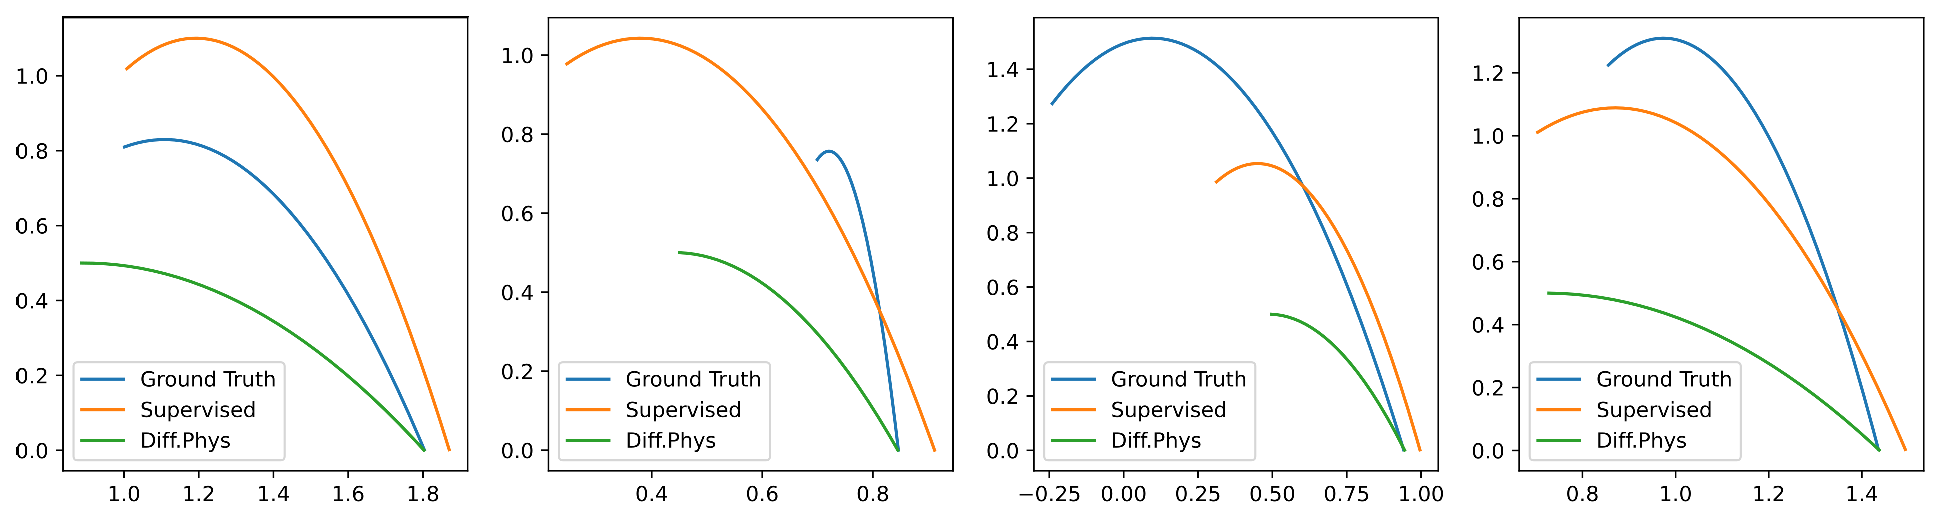
\includegraphics[width=\textwidth]{figures/throwing_results}
  \caption{Learning to throw. The goal is to give an initial velocity $v$, angle
    $\alpha$, and position $\vb{x}$ for a projectile, that hits a target at the
    ground floor when simulated.  The supervised network is outperformed by the
    \ac{DP} approach, as it always hits closer to the target by orders of
    magnitude than its supervised counterpart.  The only difference between the
    two models is the way they derive their gradients from the same $L_2$
    error: while the \ac{DP} network gains an understanding of the underlying
    physical system via gradients of the simulation, the supervised network only
    sees examples of input-output pairs, where multimodality becomes an inherent
    problem.  (Figure recreated after \citet{LearnToThrow}.)
  }
    \label{fig:learning-to-throw}
\end{figure}

\section{Reduced Order Physical Simulations}
High-dimensional data usually exhibits lower-dimensional
structure.

\todo[inline]{examples of SVD, Fourier transform on images, and on curl fields}

Although we can see that a lower-dimensional representation can yield comparable
details, simulating the evolution in this representation is usually not
straightforward.

Frame the problem as learning $f_{\text{encoder}}$,
$f_{\text{decoder}}$, and $f_{\text{time integration}}$ functions.

NNs can learn these functions.
\todo{Introduce NN approximations for these functions}

The change-of-basis, as well as time advancement operators can also be deduced
in an analytical fashion. In section~\ref{section:laplacian-eigenfluids}, we
will look at this method applied to simulating fluid dynamics in
a reduced-dimensional space.




\chapter{Fluid Simulation}\label{chapter:fluid-simulation}
Simulating convincing fluid dynamics is a continuing challenge of computer
graphics, especially when considering real-time applications. There are multiple
established ways to simulate fluids, the most widespread being Eulerian (i.e.
grid-based) and Lagrangian (i.e. particle-based) methods. Here, we restrict
ourselves to discussing Eulerian methods, and also introduce the Laplacian
Eigenfunction method, introduced by \citet{dewitt}.

The dynamics of fluids are governed by the Navier-Stokes Equations:
\begin{equation}\label{eq:NSE}
    \pdv{\vb{u}}{t} + (\vb{u}\cdot\grad)\vb{u}
    = -\frac{1}{\rho}\grad{p} + \nu\grad^2\vb{u} + \vb{f},
\end{equation}

where $\vb{u}$ is the velocity of the fluid, $\rho$ is the density, $p$ is the
scalar pressure field, $\nu$ is the viscosity constant, and $\vb{f}$ denotes
external forces. For incompressible fluids, the divergence-freeness also has to
hold, i.e. $\div{\vb{u}} = 0$

Even though equation~\eqref{eq:NSE} already describes the evolution of the fluid
as a \acf{PDE}, it is too complex for simply stepping it forward in time with
Euler steps. Instead, a technique called \textit{operator splitting} is applied
for numerical simulations, where each term is treated individually, and their
effect is combined to fully approximate the original equation. We give
a short overview of each term to get a general understanding of fluid
simulation, first treating the problem in an Eulerian way (i.e.  sampling
$\vb{u}$ on a grid), building up our way towards the Laplacian Eigenfunction
method discussed in section~\ref{section:laplacian-eigenfluids}.  For a more
complete overview of established fluid simulation techniques, see
\cite{FluidNotes} and \cite{BridsonFluid}.

Equation~\eqref{eq:NSE} is usually split by separating out the advection part,
the external force part, and the pressure/incompressibility part. When viscosity
is important, that can also be separated. This means, we work out methods for
solving these simpler equations:
\begin{align*}
    \dv{q}{t} &= 0              \qq{(advection)}\\
    \pdv{\vb{u}}{t} &= \vb{f}   \qq{(external forces)}\\
    \pdv{\vb{u}}{t} + \frac{1}{\rho}\grad p &= 0 \\
    \qq{such that}\div{\vb{u}} &= 0.
                                \qq{(pressure, enforcing incompressibility)}
\end{align*}

A generic quantity $q$ is used in the advection equation, because as we also
show later on in our experiments, we may be interested in advecting other field
quantities than just the velocity $\vb{u}$. For the advection part, the
$\text{Advect}(\vb{u}, \Delta t, q)$ algorithm is introduced: it advects
quantity $q$ through the velocity field $\vb{u}$ for a time interval $\Delta t$. 

For the external forces, any traditional numerical integration approach, such as
a simple Euler step can be used: $\vb{u}^{t+1} = \vb{u}^t + \Delta t \vb{f}$.
(See section~\ref{section:numerical-integration}.)

For calculating the pressure, an algorithm $\text{Project}(\Delta t, \vb{u})$
calculates and applies just the right amount of pressure to the velocity field
to make it divergence-free, and also enforce any solid wall boundary
conditions. The term "project" comes from the fact that the algorithm
essentially projects $\vb{u}$ to the closest divergence-free velocity field, and
interpreting the difference between these two fields as a pressure resulting
from "particles" being too close together. We do not go into the details of a
pressure solve here, as our velocity field $\vb{u}$ from the Laplacian
Eigenfunction method (section~\ref{section:laplacian-eigenfluids}) will already
be divergence-free by construction. 

Note that the order in which these algorithms are being applied matters a lot,
as the advection must be done on a divergence-free field. Putting all of these
together, a basic fluid simulation algorithm can be written as:

\begin{algorithmic}
    \State $\vb{u}^0 \gets \text{an initial divergence-free velocity field}$
    \For{$t = 0, 1, 2 \dots $}
        \State $\Delta t 
            \gets \text{a suitable time step to go from $t_n$ to $t_{n+1}$}$
        \State $\widetilde{\vb{u}} 
            \gets \text{Advect}(\vb{u}^n,\Delta t, \vb{u}^n)$
        \State $\widetilde{\vb{u}} 
            \gets \widetilde{\vb{u}} + \Delta t \vb{f}$
        \State $\vb{u}^{n+1}
        \gets \text{Project}(\widetilde{\vb{u}},\Delta t)$
            \EndFor \Comment{$[\vb{u}^0, \dots, \vb{u}^t]$ is the simulated
            fluid flow for $t$ time steps.}
\end{algorithmic}

\subsection*{Advect}
Before moving on, we briefly discuss the Advect algorithm on grids. As already
shown in section~\ref{eq:material-derivative}, we can write out the advection 
$\dv{q}{t}$ in 3D as
$$\pdv{\vb{u}}{t}\dv{t}{t} 
                    + \pdv{\vb{u}}{x}\dv{x}{t} 
                    + \pdv{\vb{u}}{y}\dv{y}{t} 
                    + \pdv{\vb{u}}{z}\dv{z}{t}$$

A simple and physically-motivated advection approach, called the semi-Lagrangian
method was introduced by \citet{StableFluids}.  Advection in a Lagrangian frame
is trivial: moving particles through a velocity field $\vb{u}$ automatically
solves $\dv{q}{t} = 0$. (Which is something we will fundamentally base our
experiments on in chapter~\ref{chapter:controlling-laplacian-eigenfluids}.) 

To find a new value $q$ at some point $\vb{x}$ in space, the semi-Lagrangian
method conceptually finds the particle, that ended up there from the previous
time step. As we know that the ``particle'' ended up at $\vb{x}$ from the previous
time step, we can trace it backwards through the velocity field to find where it
came from, grabbing the old value of $q$ at that previous point. When simulating
on a grid, but the start point was not on the grid, then interpolation is
applied.

For tracing a particle at position $\vb{x}$ \textit{backwards} in time by
$\Delta t$ through a velocity field $\vb{u}$, we can utilize integration schemes
introduced in section~\ref{section:numerical-integration}.  The simplest way is
an Euler step: 

$$\vb{x}_{\text{old}} = \vb{x} - \Delta \vb{u}(\vb{x}).$$

In practice, it is advised to apply at least a midpoint method: 
\begin{align*}
    \tilde{\vb{x}} &= \vb{x} - \frac{1}{2}\Delta t \vb{u}(\vb{x})\\
    \vb{x}_{\text{old}} &= \vb{x} - \Delta t \vb{u}(\tilde{\vb{x}}).
\end{align*}

Once we calculated $\vb{x}_{\text{old}}$, we can now simply grab the value of
$q$ from the previous time step from there, and assign it to our new position in
the current time step, i.e. $q^{t}(\vb{x}) = q^{t-1}(\vb{x}_{\text{old}})$.

For our smoke simulation examples in
chapter~\ref{chapter:controlling-laplacian-eigenfluids} , we are using
a MacCormak advection scheme \cite{maccormack} that uses a forward as well as
a backward lookup to estimate and correct the error of the semi-Lagrangian
advection.

\section{The Laplacian Eigenfunction Method}
\label{section:laplacian-eigenfluids}
\citet{dewitt} introduced the method of using Laplacian eigenfunctions for fluid
simulation. \citet{scalable-eigenfluids} addressed scalability and generalization
issues, and referred to the technique as \textit{eigenfluids}, which we also
adhere to.

The main idea is to express the velocity field $\vb{u}(\vb{x})$ via the linear
combination of $N$ global functions:

\begin{equation}\label{eq:u-lin-comb}
\vb{u}(\vb{x})=\sum_i^N w_i \Phi_i(\vb{x}),
\end{equation}

where the elements of $\vb{w} = [w_0, \dots, w_N]$ are called \textit{basis
coefficients}, and ${\Phi_i}$ are \textit{basis functions}.

As our basis functions, we choose eigenfunctions of the vector Laplacian
operator $\Delta = \grad^2 = \text{grad}(\text{div}) - \text{curl}^2$ (see
section~\ref{section:vector-laplacian}), which further simplifies to $\grad^2
= -\text{curl}^2$ for divergence-free fields.


Besides being eigenfunctions of the vector Laplacian operator, if we further
require our basis fields $\Phi_{\vb{k}}$ to be divergence-free, and to satisfy
a free-slip boundary condition, our basis functions are fully characterized by
\begin{align*}
\nabla^2 \Phi_{\textbf{k}} &= \lambda_{\textbf{k}}\Phi_{\textbf{k}} \\
\nabla \cdot \Phi_{\textbf{k}} &= 0 \\
\Phi_{\textbf{k}} \cdot \textbf{n} &= 0 \text{ at } \partial D,
\end{align*}
where $\textbf{n}$ is the normal vector at boundary $\partial D$.

Closed-form expressions of $\Phi_{\vb{k}}$ exist on the two dimensional $D \in
[0, \pi] \times [0, \pi]$ square domain \cite{chengfield}. Notating the two
scalar components in the $x$ and $y$ directions $\Phi_{\vb{k}} =(\Phi_{\vb{k},
x}, \Phi_{\vb{k},y})$, we can write them as
\begin{align*}\label{eq:explicit-u}\numberthis
    \Phi_{\vb{k},x}(x, y) &= \eta_{\vb{k}}
    \big( k_2 \sin(k_1 x) \cos(k_2 y) \big) \\
    \Phi_{\vb{k},y}(x, y) &= -\eta_{\vb{k}}
    \big( -k_1 \cos(k_1 x) \sin(k_2 y) \big),
\end{align*}

where $\vb{k} = (k_1, k_2) \in \mathbb{Z}^2$ is the \textit{vector wave number},
$\lambda_{\vb{k}} = -(k_1^2 + k_2^2)$ is the \textit{eigenvalue}, and
$\eta_{\vb{k}} = \frac{1}{-\lambda_{\vb{k}}} = \frac{1}{k_1^2 + k_2^2}$ is
a normalization parameter.  \citet{scalable-eigenfluids} use
$\frac{1}{\sqrt{-\lambda}} = \frac{1}{\sqrt{k_1^2 + k_2^2}}$ for normalization,
but we keep the non-root version, as we did not observe any noticeable
difference between the two during implementation.

As an example, $\Phi_{(4,3)}(x,y)$ is visualized in figure~\ref{fig:phi-example}.
In appendix~\ref{appendix:first_16}, we also plot the first $16$ basis fields.

This is a good time to mention that higher wave lengths corresponding to smaller
scales of vorticity has a very literal meaning in our simulation. As we choose
to truncate the spectrum of ${\Phi_k}$ at some number $N$, the error we incur is
well defined: we lose the ability to simulate vortices smaller than a given
scale. Also, as we will see later on, this correspondence to spatial scales of
vorticity lets us control the viscosity (i.e. energy decay) in relation to the
scales of vortices by modifying the base coefficients. By setting the magnitude
of each basis coefficient to decay with a time constant equal to the eigenvalue,
we get the physically correct behavior that small vortices dissipate faster than
large vortices.

\begin{figure}
  \centering
  \begin{subfigure}[t]{0.48\textwidth}
    \centering
    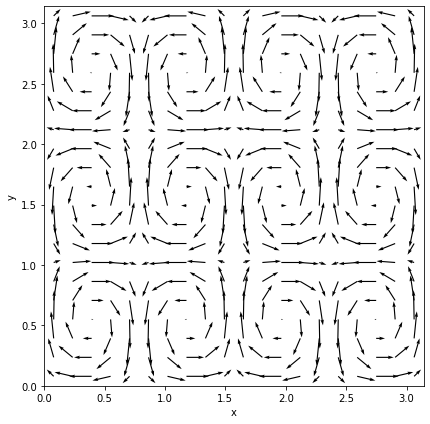
\includegraphics[height=\textwidth]{figures/eigenfluids/k_4_3_vel.png}
    \caption{Velocity field $\Phi_{(4,3)}$.}
  \end{subfigure}
  \begin{subfigure}[t]{0.48\textwidth}
    \centering
    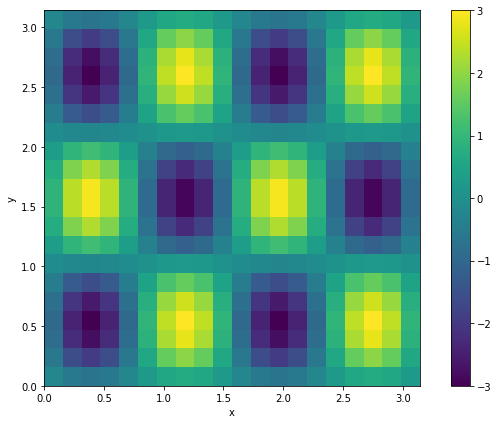
\includegraphics[height=\textwidth]{figures/eigenfluids/k_4_3_curl_bar.png}
    \caption{Curl field $\curl{\Phi_{(4,3)}} = \phi_{(4,3)}$.}
  \end{subfigure}\par\medskip
  \caption{Visualizing $\Phi_{(4,3)}$ sampled on a $20 \times 20$ grid in
  our simulation domain $D = [0,\pi] \times [0,\pi]$.}
  \label{fig:phi-example}
\end{figure}

\subsection*{Vorticity Basis Fields}
For the simulation technique, we further require the vorticity field
$\boldsymbol\omega = \curl{\vb{u}}$ and a set of vorticity basis functions $\phi
= \curl{\Phi}$.  Taking the curl (as introduced in section~\ref{section:curl})
of the velocity basis fields $\Phi_{\vb{k}}$ from equation~\eqref{eq:explicit-u}
gives us the vorticity basis fields:
\begin{align*}
    \phi_{\vb{k}} &= \curl{\Phi_{\vb{k}}} 
    =  \pdv{\Phi_{\vb{k},y}}{x} - \pdv{\Phi_{\vb{k},x}}{y}\\
&= -\mu_{\vb{k}} k_1 \sin(k_2 y) k_1(-sin(k_1 x)) - \mu_{\vb{k}} k_2 \sin(k_1 x)
    k_2 (-\sin(k_2 y))\\
&= \mu_{\vb{k}} \sin(k_1 x) \sin(k_2 y)(k_1^2+k_2^2) = \sin(k_1 x) \sin(k_2 y)
\end{align*}

We can also interpret this value as the third component of a 3D vector,
\begin{equation}
\label{eq:vorticity-basis}
\phi_{\vb{k}} = \curl{\Phi_{\vb{k}}} 
= \mqty(0 \\ 0 \\ \sin(k_1 x) \sin(k_2 y)).
\end{equation}

As the velocity field $\vb{u}$ and vorticity field $\boldsymbol{\omega}$ are
orthogonal, the vorticity basis functions $\phi_{\vb{k}}$ have only a normal
component at the boundary, and satisfy

\begin{align}
    \grad^2{\phi_{\vb{k}}} &= \lambda_{\vb{k}}\phi_{\vb{k}}\\
    \phi_{\vb{k}} \cross \vb{n} &= 0 \text{ at } \partial D.
\end{align}

\subsection*{Dynamics}
The vorticity formulation of the \eqref{eq:NSE} Navier-Stokes equation is
\begin{equation}
    \dot{\boldsymbol{\omega}} = \text{Advect}(\bf{u}, \boldsymbol{\omega}) + \nu
    \Delta\boldsymbol{\omega}
    + \curl{\bf{f}},
\label{eq:NSE-vorticity}
\end{equation}
where $\boldsymbol{\omega} = \curl{\bf{u}}$, and $\bf{f}$ denotes external
forces.

We now apply the basic building blocks of fluid simulation introduced in the
beginning of chapter~\ref{chapter:fluid-simulation} to derive the time evolution
of a fluid's velocity by the continuous change of the coefficient vector
$\vb{w}$. We derive the time derivative $\dv{\vb{w}}{t} = \dot{\vb{w}}$ in terms of
only the coefficient vector $\vb{w}$.

The velocity $\vb{u}$ formed by the eigenfunctions $\Phi_{\vb{k}}$ is
intrinsically divergence free, and hence no pressure projection step is needed,
when simulating the fluid dynamics in this coordinate system.

Damping due to viscosity is given by the first-order differential equation
$\dot{w}_k = \nu \lambda_k w_k$, which corresponds to a point-wise exponential
decay similar to \cite{StableFluids}: $$w_k^{t+1} = w_k^t e^{\nu \lambda_k
\Delta t}.$$

External forces $\vb{f}$ given on the original domain $D \in [0,\pi]\times [0,
\pi]$ can be incorporated by projecting $\vb{f}$ to the velocity basis,
representing them as a base coefficient vector $\vb{f}_w$ in the coordinate
system with basis $\{\Phi_k\}$. The contribution of the external forces is then
defined as:
$$\dot{\vb{w}} = \vb{f}_w.$$

\subsection*{Advection}
Looking at equation~\eqref{eq:NSE-vorticity}, we can see that after dealing with
both viscosity and the external forces, the only right-hand term left is the
advection.

Following \citet{dewitt}, we perform projection to a Laplacian eigenfunction
basis by substituting the expansions $\boldsymbol{\omega} = \sum_i w_i \phi_i,
\vb{u} = \sum_j w_j\Phi_j$, and $\dot{\boldsymbol{\omega}}
= \sum_k\dot{w}\phi_k$ into equation~\eqref{eq:NSE-vorticity}. With rearranging
the terms through linearity of operators, we get
\begin{equation}
    \sum_k\dot{w}\phi_k
    = \underbrace{\sum_i^N \sum_j^N w_i w_j \text{Advect}(\Phi_i, \phi_j)}_{
        \text{Advection}
    }
    + \underbrace{\nu \sum_i^N \grad^2 w_i \phi_i}_{\text{Viscosity}}
    + \underbrace{\text{curl}(\vb{f})}_{\text{External forces}}.
\end{equation}

The Advect$(\Phi_i, \phi_j)$ terms represent the non-linear advection of basis
fields. As the terms are constant, we precompute them, and the basis coefficients
of the results are stored in ``a set of $\vb{C}_k$ matrices'' (\citet{dewitt}),
resulting in $N$ number of $N \times N$ matrices, or equivalently, a ``$3^{rd}$
order advection tensor $\mathfrak{C}$'' (\citet{scalable-eigenfluids}).  The
dimensions of $\vb{C}$ and $\mathfrak{C}$ are both $N \times N \times N$. In the
following, we will refer to these precomputed advection values as $N$ $\vb{C}_k$
matrices.  The respective works also propose different ways to precompute these
values.

\citet{dewitt} propose 

\begin{equation}\label{eq:Ck-dewitt}
\vb{C}_g[h, i] = \Big( \curl(\phi_h \cross \Phi_i)\Big)\cdot \phi_g.
\end{equation}

\citet{scalable-eigenfluids} improve on \eqref{eq:Ck-dewitt} by using the method
introduced by \citet{ModelReductionFluidSim}:
\begin{equation}
    \mathfrak{C}(g,h,i) = \int_D (\curl{\Phi_i})\cdot (\Phi_g \cross \Phi_h)
    \text{d}D,
\end{equation}
noting improvements such as preserving the anti-symmetry of the tensor by
construction, i.e. $\mathfrak{C}(g,h,i) = -\mathfrak{C}(h,g,i)$. 

In our implementation, we keep with computing the basis coefficients according
to equation~\eqref{eq:Ck-dewitt}, as it was working well enough for our purposes
of differentiable physics simulation. Also note that as these are just constant
values of the same dimension and used the same way, it is trivial to change them
out at will in an implementation.

\subsection*{Time Evolution Equation}
Putting it all together, the time derivative of each basis coefficient is

\begin{equation}
    \dot{w_k} = \vb{w}\vb{C}_k\vb{w} + \nu \lambda_k w_k + f_{w,k},
\label{eq:eigenfluid-time-derivative}
\end{equation}
governing all of our reduced-order fluid simulations in
chapter~\ref{chapter:controlling-laplacian-eigenfluids}.

\subsection*{Time Integration} 
Any standard numerical technique (such as the ones discussed in
section~\ref{section:numerical-integration}) can be used to integrate
equation~\eqref{eq:eigenfluid-time-derivative} forward in time. However,
\citet{dewitt} describe a preferred technique that in order to preserve kinetic
energy, renormalizes the energy of the fluid simulation after each integration
step. \citet{dewitt} show that due to the orthogonality of the basis functions,
the total kinetic energy can be calculated as a sum of squared coefficients.
With this final addition, the final algorithm that we implemented for our
experiments in chapter~\ref{chapter:controlling-laplacian-eigenfluids} can be
described as:

\begin{algorithmic}
    \State $e_1 = \sum_i^N \vb{w}[i]^2$ 
        \Comment{store kinetic energy of velocity field}
    \For{$k = 1\dots N$}
        \State $\vb{\dot{w}}[k] = \vb{w}^T \vb{C}_k \vb{w}$
        \Comment{matrix-vector products for advection}
    \EndFor 
    \State $\vb{w} \mathrel{+}= \dot{\vb{w}} \Delta t$
        \Comment{explicit Euler integration step}
    \State $e_2 = \sum_i^N \vb{w}[i]^2$ 
        \Comment{calculate energy after time step}
    \State $\vb{w} \mathrel{*}= \sqrt{e_1 / e_2}$
        \Comment{renormalize energy}
    \For{$k = 1\dots N$}
    \State $\vb{\dot{w}}[k] \mathrel{*}= e^{\lambda_k \Delta t}$
        \Comment{dissipate energy for viscosity}
    \State $\vb{\dot{w}}[k] \mathrel{+}= \vb{f}[k]$
        \Comment{add external forces}
    \EndFor.
\end{algorithmic}

\subsubsection*{Precalculating the Advection Matrices}
Before moving on, we discuss how to compute each element of the $\vb{C}_k$
matrices in an implementation.

For finding the structure coefficients of the $\vb{C}_k$ matrices, we can start
with writing out the advection operator $\text{Advect}(\Phi_i, \phi_j)
= \curl(\phi_j \cross \Phi_i)$ as
\begin{align*}
\curl(\phi_j \cross \Phi_i) = \Big(
    &\frac{1}{\lambda_i}i_1j_2\cos(i_1x)\cos(j_2y)\sin(j_1x)\sin(i_2y)\\
    &-\frac{1}{\lambda_i}i_2j_1\cos(j_1x)\cos(i_2y)\sin(i_1x)\sin(j_2y)
\Big).
\end{align*}

The trigonometric identity $\cos(\alpha)\sin(\beta)
= \frac{1}{2}\sin(\alpha+\beta)-\frac{1}{2}\sin(\alpha-\beta)$ enables factoring
to a suitable expression which is in the span of $\{\phi_k\}$:
\begin{align*}
\text{Advect}(\Phi_i,\phi_j)= \frac{1}{4\lambda_{i}}
    \Big[&(i_1 j_2 - i_2 j_1)\phi_{i_1+j_1, i_2+j_2}\\
     &-(i_1 j_2 + i_2 j_1)\phi_{i_1+j_1, i_2-j_2}\\
     &+(i_1 j_2 + i_2 j_1)\phi_{i_1-j_1, i_2+j_2}\\
     &-(i_1 j_2 - i_2 j_1)\phi_{i_1-j_1, i_2-j_2}\Big].\\
\end{align*}

The resulting coefficients are\footnote{Deriving the underlying equations by
hand, and consulting the original implementation by \citet{dewitt}, one of the
signs is purposefully different from the appendix in \cite{dewitt}.}
\begin{align*}\numberthis\label{eq:structure-coeff-values}
    \vb{C}_{i_1+j_1,i_2+j_2}[i,j] &= -\frac{1}{4(i_1^2 - i_2^2)}(i_1j_2-i_2j_1)\\
    \vb{C}_{i_1+j_1,i_2-j_2}[i,j] &= \frac{1}{4(i_1^2 + i_2^2)}(i_1j_2+i_2j_1)\\
    \vb{C}_{i_1-j_1,i_2+j_2}[i,j] &= -\frac{1}{4(i_1^2 + i_2^2)}(i_1j_2+i_2j_1)\\
    \vb{C}_{i_1-j_1,i_2-j_2}[i,j] &= \frac{1}{4(i_1^2 - i_2^2)}(i_1j_2-i_2j_1).\\
\end{align*}

\textbf{Note:} We are using $\vb{k} = (k_x, k_y) = (k_1, k_2)$ interchangeably.
A single (non-vector) $k$ is also used for indexing over all of the basis fields
-- a slight, but very useful abuse of notation, stemming from the fact that
a suitable remapping from vector wave lengths $(k_1, k_2)$ to positive integers
is necessary in an implementation, as seen in the indexing of the $\vb{C}_k$
values in \eqref{eq:structure-coeff-values} above.

\chapter{Controlling Laplacian Eigenfluids}
\label{chapter:controlling-laplacian-eigenfluids}
Many real world applications require us to optimize for some parameters of
a physics-based problem. A toy example would be to optimize for some initial
angle and velocity of a projectile to hit some target (see
figure~\ref{fig:learning-to-throw}). As a more involved example, \citet{MinDrag}
address finding the best shape to minimize drag. These kinds of inverse problems
have been around for quite some time in engineering applications.

Building on all of the previous ideas, we now introduce our investigation into
the use of eigenfluids in fluid control problems, making use of their explicit
closed-form description of a velocity field (equation~\eqref{eq:explicit-u}) to
derive gradients used for optimization. Our main proposition is to achieve
reduced-order modeling-like speed increase: in lieu of representing the fluid on
a grid, we reconstruct the velocity field only at discrete points in space,
while simulating the dynamics of the fluid in a reduced dimensional
space as in equation~\eqref{eq:u-lin-comb}.

In the following, we showcase different optimization scenarios, where we try out
different aspects of controlling eigenfluids via \acf{DP} gradients. (See
section~\ref{dp-loss}.)

We start with examples of "traditional" optimization scenarios. By
"traditional", we mean finding individual solutions to problems via some
optimization technique -- in our case, \acf{GD}. Moving further, we look for
generalized solutions to a set of problems by training \acfp{NN}.

After trying out multiple recent frameworks aimed at differentiable simulations
\cite{warp2022,difftaichi}, we implemented all of our experiments
using $\Phi_{Flow}$ \cite{holl2019pdecontrol}.

\section{Matching Velocities}\label{section:matching-velocities}
To verify the feasibility of our technique before moving on to more involved
setups, our most straightforward optimization scenario is finding an initial
basis coefficient vector $\vb{w}_0 \in \mathbb{R}^N$ for an eigenfluid
simulation using $N=16$ basis fields, such that when simulated for $t$ time
steps, the reconstructed $\mathcal{R}\vb{w}_t = \vb{u}_t$ velocity
field will match some precalculated $\vb{u}^*: [0,\pi]\times[0,\pi] \to
\mathbb{R}^2$ target velocity field:

\begin{equation}\label{eq:match-vel-loss}
  L(\vb{w}) = \left|
  \mathcal{R}\mathcal{P}^{t}(\vb{w}) - \vb{u}^*
  \right|_2^2,
\end{equation}

where $\mathcal{P}^t(\vb{w}) = \mathcal{P} \circ \mathcal{P} \dots \circ
\mathcal{P}(\vb{w})$ is the physical simulation of base coefficients $\vb{w}$
(in the reduced dimension) $t$ times.

For the optimization, we initialize a $\vb{w}_\text{init} \in \mathbb{R}^N$
vector with random numbers (from a normal/Gaussian distribution), and run the
eigenfluid simulation for $t$ time steps, after which, we measure the error as
given by loss function \eqref{eq:match-vel-loss}. Relying on backpropagation to
derive the necessary gradients, we use the \ac{GD} optimization method as
introduced in equations~\eqref{eq:gd-steps} to iteratively find a vector
$\vb{w}_{optim}$, yielding a low scalar loss $L(\vb{w}_{optim})$.

To be able to make some further evaluation of the end results possible, we step
an eigenfluid solver for time $t$ to precalculate the target $\vb{u}^*$ velocity
field, sampled on a $32\times32$ grid. We denote the initial base coefficient
vector of this reference simulation $\vb{w}^*$, but keep in mind that the
optimization has absolutely zero knowledge of this value, as it sees only the
$32\times32\times2$ velocity values of $\vb{u}^*$ at time $t$. Also, these
values could have been precalculated from any other kind of fluid simulation as
well, or even just initialized randomly. Deriving $\vb{u}^*$ as the result of an
eigenfluid simulation has the added benefit of exposing to us a solution
$\vb{w}^*$ that we can use to compare with the solution of the optimizer.

We test this setup on two scenarios, with differing the number of time steps
simulated: first with $t=16$, and then with $t=100$.

For $t=16$ simulation steps, starting from a loss of around $400$, the first
$100$ \ac{GD} optimization steps with $\lambda=10^{-3}$ reduced the loss to
under $1.0$, while $200$ steps further decreased it to under $4*10^{-4}$, with
each further step still continuously decreasing the error. 

Naturally, this very basic method has its limits.  Optimizing for initial
coefficients based solely on that when reconstructed on a $32\times32$ grid
after $100$ steps of a non-linear simulation, they should match a given velocity
field, proved to be a substantially harder problem, as even a relatively small
error can accumulate into major deviations over these longer time steps,
resulting in much less stable gradients. With using the same learning rate, the
optimization diverged almost instantly. With some tuning of the learning rate
$\lambda$ in the range of $[10^{-4}, 10^{-8}]$, we were able to get the loss
below $0.14$.  (Starting from an initial loss of $320$ from the random
initialization.) 

We visualize the results of these two scenarios in
Figure~\ref{fig:matching-velocities}. It is interesting to observe that even
though the optimization had absolutely no knowledge of $\vb{w}^*$, only
a comparison with a precomputed $\vb{u^*}$ velocity field at time step $100$, the
optimized $\vb{w}_{optim}$ vector already starts to look similar to $\vb{w}^*$.
Keep in mind that this is not guaranteed at all, as highlighted with the
learning to throw example on figure~\ref{fig:learning-to-throw}. In some other
cases of running this optimization setup, we also observed $\vb{w}_{optim}$s
that are completely different from $\vb{w}^*$. Due to the physical constraints
of the eigenfluids simulation, in these cases the optimization could not change
any of the $16$ values of $\vb{w}_{optim}$ locally in a way that would further
reduce the loss below some small number, and was stuck in a local minima of the
parameter space.

Although there are a number of ways to tweak this setup, we can already verify
from these results that  the flow of the gradients is working, and is ready to
be tested in more advanced scenarios.

\begin{figure}
  \centering
  \begin{subfigure}{\textwidth}
    \centering
    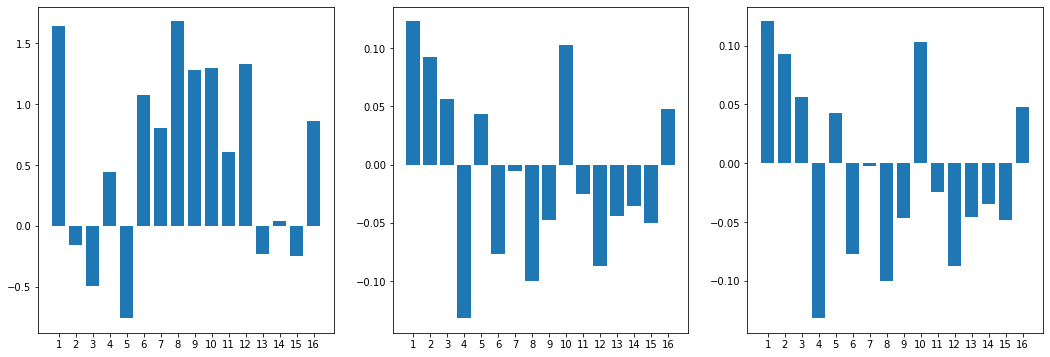
\includegraphics[width=0.9\textwidth]{figures/finding-initial-velocities/t_16_coefficients.png}
    \caption{$\vb{w}_{init}$, $\vb{w}_{optim}$, and
    $\vb{w}^*$, optimizing for velocity field after $16$ time steps}
    \label{fig:16-timesteps-coeffs}
  \end{subfigure}\par\medskip
  \begin{subfigure}{\textwidth}
    \centering
    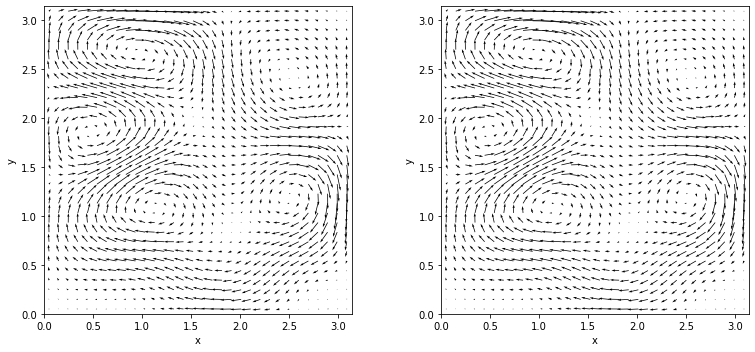
\includegraphics[width=0.8\textwidth]{figures/finding-initial-velocities/t_16_velocities.png}
    \caption{Target $\vb{u}^*$, and $\vb{u}^{16}$, reconstructed from
      $\mathcal{P}^{16}(\vb{w}_{optim})$\\}
    \label{fig:16-timesteps-vel}
  \end{subfigure}\par\medskip
  \begin{subfigure}{\textwidth}
    \centering
    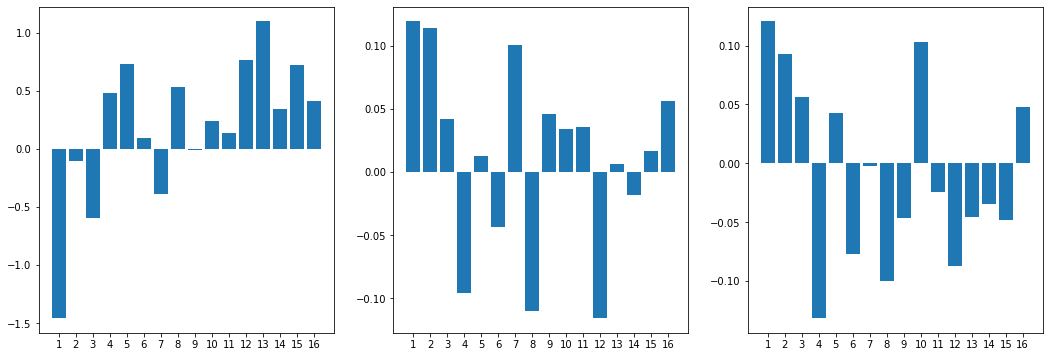
\includegraphics[width=0.9\textwidth]{figures/finding-initial-velocities/t_100_coefficients.png}
    \caption{Initial basis coefficients $\vb{w}_{init}$, $\vb{w}_{optim}$, and
    $\vb{w}^*$, optimizing for velocity field after $100$ time steps\\}
    \label{fig:100-timesteps-coeffs}
  \end{subfigure}\par\medskip
  \begin{subfigure}{\textwidth}
    \centering
    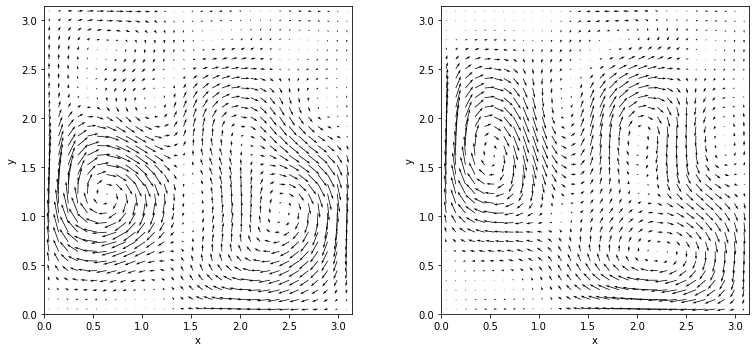
\includegraphics[width=0.8\textwidth]{figures/finding-initial-velocities/t_100_velocities.png}
    \caption{Target $\vb{u}^*$, and $\vb{u}^{100}$, reconstructed from
      $\mathcal{P}^{100}(\vb{w}_{optim})$}
    \label{fig:100-timesteps-vel}
  \end{subfigure}
  \caption{Results of optimizing for an initial $\vb{w}_0$ basis coefficient
    vector that matches a target velocity field $\vb{u}^*$ when reconstructed
    after simulating for $t$ time steps.
  }
  \label{fig:matching-velocities}
\end{figure}

\section{Controlling Shape Transitions}
\label{section:controlling-shape-transitions}
In the following, we showcase an optimization scenario, with the target of
controlling the transition between two marker shapes in a fluid simulation
setup. 
\footnote{Note that we use the terms \textit{smoke}, \textit{marker},
\textit{density}, and \textit{scalar valued density/marker function}
interchangeably throughout the text.}
The work of \citet{holl2019pdecontrol} formulated this problem in an
Eulerian representation, with explicitly simulating the shapes as scalar marker
densities being advected by the velocity field of the simulated fluid. 

Playing to the strength of the eigenfluids method, our method makes use of an
explicit, closed-form description of the fluid velocity $\vb{u}$ as in
equation~\eqref{eq:explicit-u}. We stay independent of a grid resolution, and
approximate the 2D shapes via a set of sample points. We reconstruct the
velocity field only partially at these discrete points as needed for the
advection of these particles. This results in both a faster fluid simulation as
well as optimization as compared to fully simulating an $N\times N$ grid,
advecting a marker density, and backpropagating gradients of a physical
simulation with much more degrees of freedom.

We formulate three different control problems, each with a different mean to
exert control over the fluid simulation.
\begin{itemize}
  \item First, in a similar vein to the problem statement in
    section~\ref{section:matching-velocities}, we are looking for an initial
    coefficient vector $\vb{w}_0$ of an eigenfluids simulation, such that when
    simulated for $t$ time steps, the reconstructed velocity field advects some
    initial points to the desired positions.
  \item Second, we optimize for some force vector $\vb{f}\in \mathbb{R}^{t\times
    N}$, such that $\vb{f}_t \in \mathbb{R}^N$ applied as external force to each
    time step of an eigenfluid simulation, it yields the desired outcome.
  \item Finally, we generalize the problem to looking for a function that exerts
    the necessary control force at time $t$, such that particles currently at
    positions $\vb{p}_t$ end up at target positions $\vb{p}_{t+1}$ at the
    next time step. We formulate this third task as a \acf{NN} model in the
    form $\vb{f}(\vb{p_t}, \vb{p_{t+1}}, \vb{w}_{t}, \boldsymbol\theta)$, also
    passing in the current basis coefficient vector $\vb{w}_t$, and optimizing
    for its parameters $\boldsymbol\theta$ to yield the desired outcome.
\end{itemize}

In each of these tasks, a velocity field $\vb{u} = \mathcal{R}\vb{w}$ advects
a set of initial points $\vb{p}_0 = \left[\vb{p}_0^0,\dots, \vb{p}_0^i\right]$
to line up with target positions $\vb{p}_t = \left[\vb{p}_t^0, \dots,
\vb{p}_t^i\right]$.  We formulate this as 

\begin{equation}\label{eq:advecting-particles-loss}
  L(\vb{w}, \vb{p}_0, \vb{p}_t)
  = \left| \mathcal{P}^{t}(\vb{p}_0, \vb{w}) - \vb{p}_t\right|_2^2 
  = \sum_{i}\left|\mathcal{P}^{t}(p_0^i, \vb{w}) - p_t^i\right|_2^2, 
\end{equation}

where $\mathcal{P}^t(\vb{w}, \vb{p}) = \underbrace{\mathcal{P} \circ
\mathcal{P}\circ \dots \circ \mathcal{P}(\vb{w}, \vb{p})}_{t \text{ times}}$
denotes the physical simulation of base coefficients $\vb{w}$ and points
$\vb{p}$ in $\vb{u} = \mathcal{R}\vb{w}$, the velocity field reconstructed from
$\vb{w}$.  We use a simple mean-square error (also known as squared $L_2$ norm)
for measuring the error.

\subsection{Sampling}\label{section:sampling}
Advection of some scalar quantity in a fluid is an abstract problem that
describes many real-world phenomena. We can think of the transport of some ink
dropped into water, clouds in the air, or some buoyant smoke rising. Phenomena
such as these can be modeled as a density function $\psi(\vb{x})$ defined over
the simulation domain $D$. In a fluid with velocity $\vb{u}$, and $\div{\vb{u}}
= 0$ (i.e. the fluid is incompressible), the advection is governed by the
equation

$$\pdv{\psi}{t} + \vb{u}\cdot \grad{\psi} = 0.$$

In Eulerian fluid simulation methods \cite{StableFluids}, both
$\vb{u}$ and $\vb{\psi}$ are sampled on grids, numerically approximating the
evolution of the field quantities. Instead, our method proposes sampling the
density function at discrete particle positions, thus rephrasing the process in
a Lagrangian way.

In the context of Laplacian eigenfluids, a Lagrangian viewpoint is especially
inviting, as the explicit description of the fluid velocity $\vb{u}$
(equation~\eqref{eq:explicit-u}) allows us to reconstruct $\vb{u}$ only
partially, while keeping the simulation of the fluid dynamics in a reduced
dimensional space. In a forward physics simulation, this can already lead to
substantial speed-ups, but this formulation seems especially promising when the
backpropagation of variables is desired, such as the optimization scenarios
introduced herein.

A straightforward way to define a shape is
\begin{equation}\label{eq:binary-shape-function}
\psi(\vb{x}) = 
\begin{cases}
  1, & \qq*{inside the shape}\\
  0, & \text{outside the shape}.\\
\end{cases}
\end{equation}
Sampled on an $N \times N$ grid, this is equivalent to a binary image with
a resolution of $N \times N$. Moreover, when sampled on a grid, and advected,
it is straightforward to interpret the resulting grid and its values as
a grayscale image with values $[0,\dots,1]$.

Often used in 3D scanning, reconstruction and scene understanding problems,
a \acf{SDF} can be defined as the distance to the surface (in 2D, the edge) of
an object, with positive values outside, and negative values inside. In our
implementation, we define our shapes as \acp{SDF}. For example, a circle with
radius $r$ and center $\vb{o} = (o_x, o_y)^T$ is defined as

$$\text{SDF}_{\text{circle}}(\vb{x, \vb{o}, r}) 
  = \abs{\vb{x}-\vb{o}} - r
  = \sqrt{(x-o_x)^2 + (y-o_y^2)} - r.$$

For simulating (and visualizing) the advection dynamics of these shapes, we
transform the SDFs to a binary form as in
equation~\eqref{eq:binary-shape-function}.

As we neither want to lose too much information about our original function, nor
want to keep track of an unnecessary number of points, the feasibility of this
method necessitates an efficient sampling of $\psi(\vb{x})$. We use a simple
rejection-based sampling technique. Transforming the shapes to fit inside the
unit rectangle $[0,1]\times[0,1]$, we generate random points
$\vb{p}_\text{sample}\in [0,1]\times[0,1]$, rejecting them if they lie outside
the shape.

As we consider shape transitions given start and target shapes $S_\text{0}$ and
$S_\text{t}$, it is important to take into consideration the connection between
these shapes. To balance finding spatial correspondences between the shapes,
while still approximating their unique shapes, we sample $O$ overlapping, and
$U$ unique points. For the overlapping points, we accept only
$\vb{p}_\text{sample} \in S_\text{0} \cup S_\text{t}$, i.e. we reject points
that are not inside both shapes (transforming both shapes to fit inside the unit
square for the sampling). For the unique points we sample a different set of
points for each shape. 

To generate low-discrepancy, quasi-random 2D coordinates, we use a Halton
sequence \cite{halton}, giving deterministic coordinates, given coprimes $p$
and $q$. Using one set of primes for sampling $O$ overlapping points, and
another set of primes for sampling $U$ unique points can give us further
overlapping points, as the proposed (but potentially rejected) sequence of
points will be the same for both shapes.

We further generate $T=5$ trivial points that are hand-picked to best resemble
the given shape, as well as line up between different shapes. We choose these to
be the center, upper right, upper left, lower left, and lower right corners of
the shape. 

In conclusion, our final set of $\vb{p}_0$ initial, and $\vb{p}_t$ target sample
positions are given by concatenating the $O$ overlapping, $U$ unique, and $T$
trivial points for each shape, resulting in two set of sample points $\vb{p}_0,
\vb{p}_t \in \mathbb{R}^{O+U+T}$.

Figure~\ref{fig:sampling} shows the result of our sampling strategy for
a triangle and a circle shape.

\begin{figure}
  \centering
  \begin{subfigure}[t]{0.48\textwidth}
    \centering
    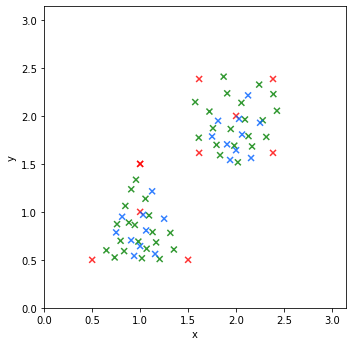
\includegraphics[width=\textwidth]{figures/sampling/points.png}
    \caption{The $O=30$ overlapping (blue), $U=30$ unique (green), and $T=5$
    trivial (red) points for each shape.}
  \end{subfigure}
  \begin{subfigure}[t]{0.48\textwidth}
    \centering
    % 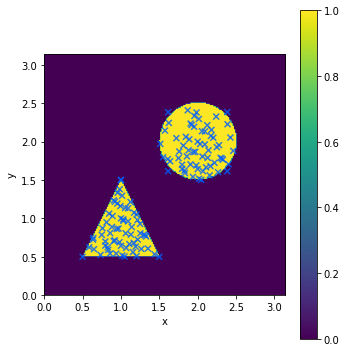
\includegraphics[width=\textwidth]{figures/sampling/smokes.png}
    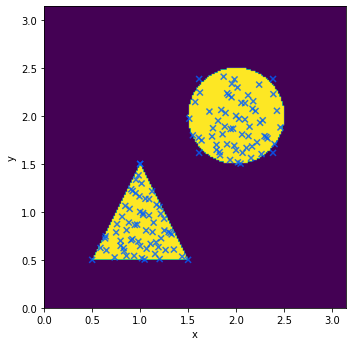
\includegraphics[width=\textwidth]{figures/sampling/smokes_no_bar.png}
    \caption{Sample points plotted over $\psi_\text{triangle}
    + \psi_\text{circle}$.}
  \end{subfigure}\par\medskip
  \caption{Sampling strategy for transitioning from a triangle to a circle.
  Halton series with base $(2,7)$ and $(3,11)$ were used to generate the
  overlapping and unique positions, respectively.}
  \label{fig:sampling}
\end{figure}

\subsection{Optimizing for Initial Velocity}\label{section:initial-velocity} 
As introduced the problem in the beginning of the chapter (see
equation~\ref{eq:advecting-particles-loss}), our goal is to find an initial
velocity field $\mathcal{R}\vb{w} = \vb{u}$ that advects points $\vb{p}_0$ to
line up with target positions $\vb{p_t}$ after $t$ steps. 
We can write optimizing for base coefficients $\vb{w}$ as:

$$\arg\min_{\vb{w}} \left| \mathcal{P}^{t}(\vb{p}^0, \vb{w})
- \vb{p}^t\right|_2^2.$$

Making use of the differentiability of our physical simulator $\mathcal{P}$, and
the multivariable chain rule for deriving the gradient of the above
$\mathcal{P}^t = \mathcal{P}\circ\dots\circ\mathcal{P}$ function composition, we
can derive its gradient with respect to the initial coefficients:
$$\frac{\partial \mathcal{P}^t(\vb{w},\vb{p})}{\partial \vb{w}}.$$

Finally, as introduced in \eqref{eq:gd-steps}, we simply iterate a \ac{GD}
optimizer to find a (good enough) solution for our above minimization problem:

$$\vb{w}_{\text{better}} = \vb{w} - \lambda
\frac{
    \partial L(\vb{w}, \vb{p}_0, \vb{p}_t)
}{
    \partial \vb{w}
},$$

where $L$ is the same as in equation~\eqref{eq:advecting-particles-loss}:
\begin{equation*}
  L(\vb{w}, \vb{p}_0, \vb{p}_t)
  = \left| \mathcal{P}^{t}(\vb{p}_0, \vb{w}) - \vb{p}_t\right|_2^2.
\end{equation*}

The main difficulty of this non-linear optimization problem lies in that we have
no control over the natural flow of the fluid besides supplying an initial
$\vb{w}_0$ vector.

We showcase two different setups in Figure~\ref{fig:points-vel-only}, with the
details of both experiments described in Table~\ref{table:vel-optim-details}.

\begin{table}[!h]
  \caption{Details of the 2 optimization scenarios shown in
  Figure~\ref{fig:points-vel-only}}
  \label{table:vel-optim-details}
  \centering
\begin{tabular}{r|cc}
  \multicolumn{1}{l}{}               
  & \multicolumn{1}{|l}{\textbf{Figure~\ref{fig:points-vel-only-small}}}
  & \multicolumn{1}{l}{\textbf{Figure~\ref{fig:points-vel-only-big}}}\\ \hline
N                                  & 16                                     & 36                                     \\ \hline
Sampling size for smoke simulation & 32                                     & 32                                     \\ \hline
Eigenfluid initialization time     & 6.19 sec                               & 68.47 sec                              \\ \hline
Time for 51 optimization steps     & 108.05 sec                             & 230.48 sec                             \\ \hline
Initial loss                       & 2.3                                    & 2.19                                   \\ \hline
Final loss                         & 0.08                                   & 0.09                                   \\ \hline
Number of overlapping points $O$                                  & 0                                      & 30                                     \\ \hline
Number of unique points $U$                                  & 0                                      & 30                                     \\ \hline
Number of trivial points $T$                                  & 5                                      & 0                                      \\ \hline
\end{tabular}
\end{table}
\begin{figure}
  \centering
  \begin{subfigure}{\textwidth}
    \centering
    \begin{subfigure}{0.4\textwidth}
      \centering
      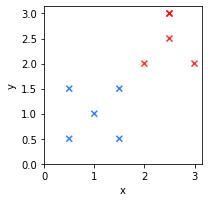
\includegraphics[width=0.7\textwidth]{figures/points-velocity-only/T5/start_target.png}
      \caption{$O=0$, $U=0$, $T=5$} 
    \end{subfigure}
    \begin{subfigure}{0.4\textwidth}
      \centering
      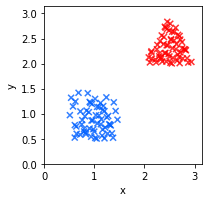
\includegraphics[width=0.7\textwidth]{figures/points-velocity-only/O30_U30_T0/start_target.png}
      \caption{$O=30$, $U=30$, $T=0$}
    \end{subfigure}
    \caption{Initial (blue), and target (red) sample points.}
  \end{subfigure}\\
  \begin{subfigure}{\textwidth}
    \centering
    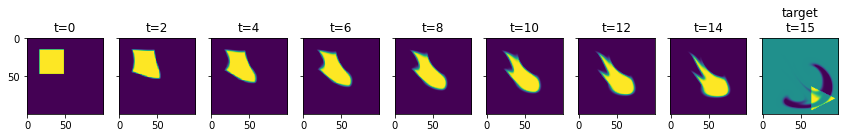
\includegraphics[width=\textwidth]{figures/points-velocity-only/T5/trajectory_horizontal.png}
    \caption{Using $N=16$ basis fields, and the $T=5$ trivial points.}
    \label{fig:points-vel-only-small}
  \end{subfigure}\\
  \begin{subfigure}{\textwidth}
    \centering
    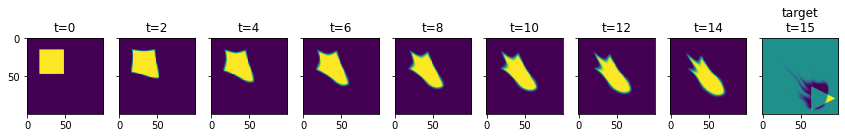
\includegraphics[width=\textwidth]{figures/points-velocity-only/O30_U30_T0/trajectory_horizontal.png}
    \caption{Using $N=36$ basis fields, and using a total of $60$ sampling
    points.}
    \label{fig:points-vel-only-big}
  \end{subfigure}\\
  \caption{Solving the shape transition problem by optimizing for an initial
  coefficient vector $\vb{w}$ without any further control over the simulation.}
  \label{fig:points-vel-only}
\end{figure}

\subsection{Control Force Estimation}\label{section:cfe}
In this scenario, we optimize for a force vector $\vb{f} \in \mathbb{R}^{t\times
N}$, such that $\vb{f}_t \in \mathbb{R}^N$ applied as external force at each
time step of an eigenfluid simulation, some initial positions $\vb{p}_0$ will be
advected to target positions $\vb{p}_t$ after $t$ time steps:

$$\arg\min_{\vb{f}} \left| \mathcal{P}^{t}(\vb{p}_0, \vb{w}, \vb{f})
  - \vb{p}_t\right|_2^2,$$

where $\mathcal{P}^{t}(\vb{p}_0, \vb{w}, \vb{f}) = \mathcal{P} \circ \dots
\circ \mathcal{P}(\vb{p}_0, \vb{w}, \vb{f})$ denotes simulating the
physical system for $t$ time steps, applying $\vb{f}_t$ force at each
time step.

Results of the optimization are shown in Figure~\ref{fig:f_optim}.

\begin{figure}
  \centering
  \begin{subfigure}{\textwidth}
    \centering
    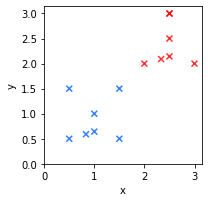
\includegraphics[width=0.3\textwidth]{figures/f-optim/blue_start_red_target.png}
    \caption{Initial (blue), and target (red) sample points. ($O=1$, $U=1$,
    $T=5$)}
  \end{subfigure}\\
  \begin{subfigure}{\textwidth}
    \centering
    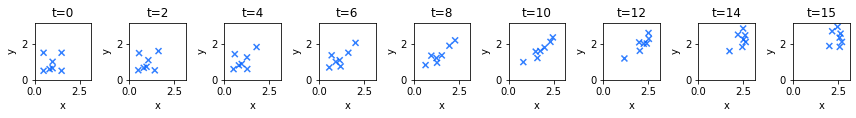
\includegraphics[width=\textwidth]{figures/f-optim/trajectory_horizontal.png}
    \caption{Optimized trajectory of the sample points underlying the
    optimization.}
  \end{subfigure}\par\medskip
  \begin{subfigure}{\textwidth}
    \centering
    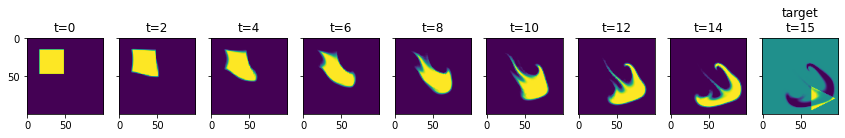
\includegraphics[width=\textwidth]{figures/f-optim/smoke_trajectory_horizontal.png}
    \caption{Smoke advection for qualitative comparison, reconstructed on
    a $100\times 100$ grid.}
  \end{subfigure}\par\medskip
  \caption{Force optimization results with $16$ time steps, and using $N=16$
  basis fields.}
  \label{fig:f_optim}
\end{figure}

\pagebreak
\subsection{Neural Network Training}\label{section:nn-training}
We generalize the \acf{CFE} problem by defining a function
$\vb{f}(\vb{p}_0,\vb{p}_t,\vb{w}): \mathbb{R}^{2\cdot2(O+U+T)+N}\to
\mathbb{R}^N$, that gives a force vector $\vb{f} \in \mathbb{R}^N$ to be
applied at the current time step to move points $\vb{p}_0$ to $\vb{p}_t$ in the
next time step. Its inputs are the $(x,y)$ coordinates of $\vb{p}_0$ and
$\vb{p}_t$, as well as the basis coefficient vector $\vb{w}$ at the current
time step concatenated after each other, giving $2\cdot2(O+U+T)+N$ values, where
$O$, $U$, and $T$ denote the number of overlapping, unique, and trivial sample
points, respectively, as introduced in section~\ref{section:sampling}.

We approximate the \ac{CFE} function $\vb{f}$ with a Control Force Estimator
\acf{NN} $\vb{f}(\vb{p}_0, \vb{p}_t, \vb{w}, \vb{\theta})$. 

Each layer is constructed exactly as described in
equation~\eqref{nn-single-layer-math} with ReLU non-linearities, making the
resulting concatenation of layers the same as in
equation~\eqref{eq:nn-layers-math}. Figure~\ref{fig:nn-architecture} gives an
overview of our \ac{NN} architecture. 

\begin{figure}[h]
  \centering
  \hspace*{-0.75cm}
  \begin{tikzpicture}
    \node (x) at (0,0) {\small$[\vb{p}_0, \vb{p}_t,\vb{w}]$};
 
    \node[conv,rotate=90,minimum width=4.5cm] (l0) at (2,0) 
      {\small Linear + ReLU};

    \node[conv,rotate=90,minimum width=4.5cm] (l1) at (4.0, 0)
      {\small Linear + ReLU};

    \node[conv,rotate=90,minimum width=4.5cm] (l2) at (6.0, 0)
      {\small Linear + ReLU};

    \node[conv,rotate=90,minimum width=4.5cm] (l3) at (8.0, 0)
      {\small Linear + ReLU};

    \node[conv,rotate=90,minimum width=4.5cm] (l4) at (10.0, 0)
      {\small Linear + ReLU};

    \node[conv,rotate=90,minimum width=4.5cm] (l5) at (12.0, 0)
      {\small Linear + ReLU};
    
      \node (f) at (13.5,0) {\small$\vb{f}$};
    
      \draw[->] (x) -- (l0);
    \draw[->] (l0) -- (l1) node[pos=0.5,sloped,above] {$512$};
    \draw[->] (l1) -- (l2) node[pos=0.5,sloped,above] {$256$};
    \draw[->] (l2) -- (l3) node[pos=0.5,sloped,above] {$128$};
    \draw[->] (l3) -- (l4) node[pos=0.5,sloped,above] {$64$};
    \draw[->] (l4) -- (l5) node[pos=0.5,sloped,above] {$32$};
    \draw[->] (l5) -- (f) node[pos=0.5,sloped,above] {$16$};
    
  \end{tikzpicture}
  \vskip 6px
  \caption{The CFE NN transforms the input vector of size $2\cdot2(O+U+T)+N$
  into a force vector $\vb{f}$ that can be added to the $\vb{w}$ coefficients as
external force. The output size of each layer matches the input size of the
following layer, and a ReLU non-linearity is applied after each layer.}
  \label{fig:nn-architecture}
\end{figure}


As the input size to the \ac{NN} is dependent on the specific problem, the
number of trainable parameters also varies, and a new \ac{NN} has to be trained
when using a different number of basis fields, or different number of total
sample points. As an example, for $N=16$ basis fields, and $75$ sample points,
the \ac{NN} has $337 392$ trainable parameters.

\subsection*{Overfitting to a single training sample}
Testing the setup, we overfit the \ac{NN} to a single training sample. Plotting
the results of the time evolution on figure~\ref{fig:NN-overfit}, we observe
that a reduced degrees of freedom can yield comparable, or even better results
with the same setup, and training time. 

Using an Adam optimizer \cite{adam} with learning rate $10^{-3}$, the results
shown in Figure~\ref{fig:NN-overfit} were achieved in $260$ epochs. The
training took $53.94$ seconds.

\begin{figure}
  \centering
  \begin{subfigure}{\textwidth}
    \centering
    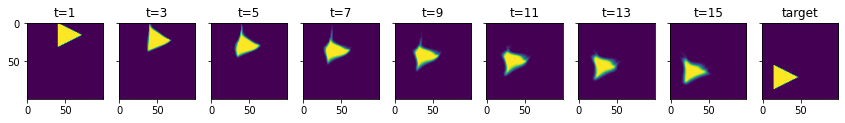
\includegraphics[width=\textwidth]{figures/nn-training/NN_N16_triangle_overfit_horizontal.png}
    \caption{$N=16$ basis fields}
  \end{subfigure}
  \begin{subfigure}{\textwidth}
    \centering
    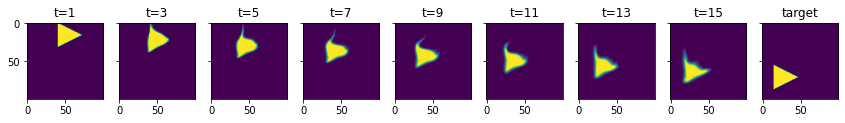
\includegraphics[width=\textwidth]{figures/nn-training/NN_N36_triangle_overfit_horizontal.png}
    \caption{$N=36$ basis fields}
  \end{subfigure}
  \caption{Time evolution of simulating two overfitted \ac{CFE} \acp{NN} to
  a single shape transition for $16$ time steps $t=[0\dots15]$. Using $O=30$
overlapping, $U=40$ unique, and $T=5$  trivial sample points.}
  \label{fig:NN-overfit}
\end{figure}

\subsection*{Training}
We generate $2000$ samples, using $1800$ for training, and $200$ for validation.
Using $N=16$ basis fields, we train the \ac{NN} for the \ac{CFE} problem
detailed above. (See Figure~\ref{fig:NN-shape-transition-train}.)

At the end of the training, we generate further data the \ac{NN} has not seen
during training to further test generalization.
(See Figure~\ref{fig:NN-shape-transition-test}.)

Using an Adam \cite{adam} optimizer with learning rate $10^{-3}$, the results
shown in Figure~\ref{fig:NN-shape-transition} were achieved in $260$ epochs. The
training took $1201.74$ seconds ($20$ minutes).

As we did not experience any overfitting issues during training, no additional
regularization schemes were applied. 

\begin{figure}
  \centering
  \begin{subfigure}{\textwidth}
    \centering
    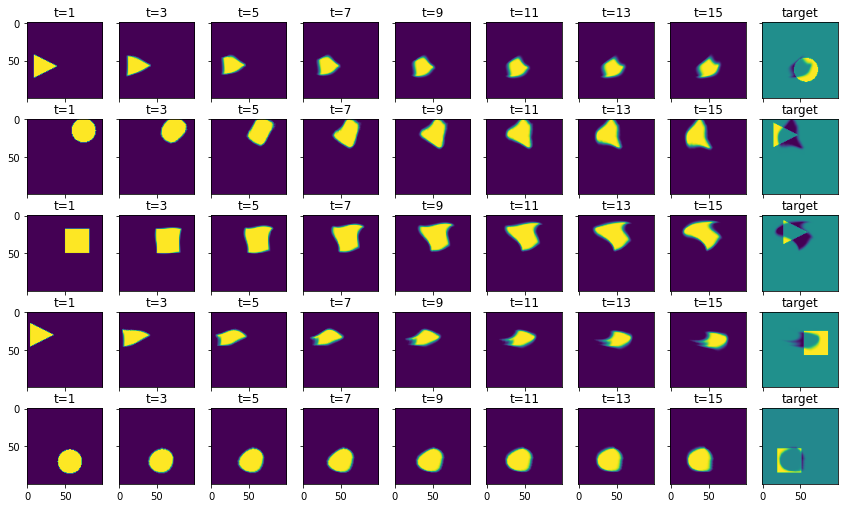
\includegraphics[width=\textwidth]{figures/nn-final/trained_trajectories_horizontal.png}
    \caption{Performance after training on the \textbf{training data}. (Randomly
    sampled.)}
    \label{fig:NN-shape-transition-train}
  \end{subfigure}
  \begin{subfigure}{\textwidth}
    \centering
    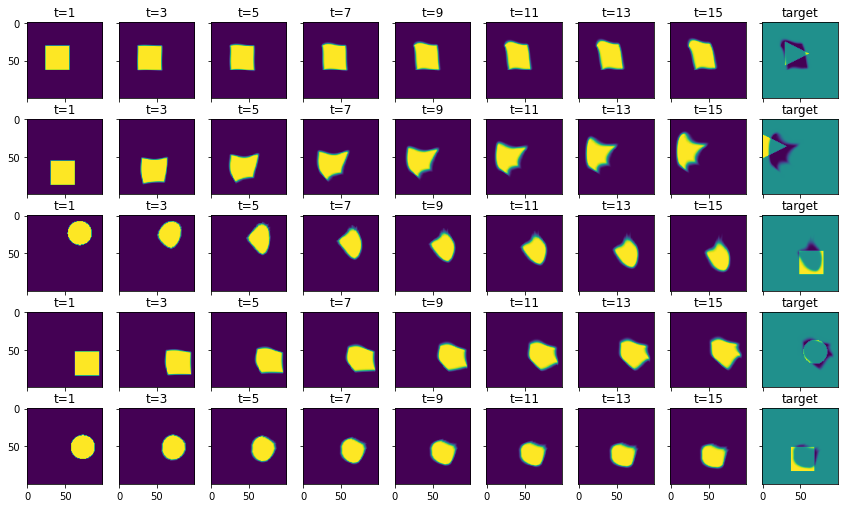
\includegraphics[width=\textwidth]{figures/nn-final/test_trajectories_horizontal.png}
    \caption{Testing on previously unseen \textbf{test data}. (Randomly
      sampled.)}
    \label{fig:NN-shape-transition-test}
  \end{subfigure}
  \caption{Randomly sampled time evolution of controlled shape transition
  tasks. Using $N=16$ basis fields, sampling the smokes on a $32\times 32$ grid,
  approximating them with $O=30$ overlapping, $U=40$ unique and $T=5$ trivial
  sample points, through $16$ time steps $t=[0\dots15]$.}
  \label{fig:NN-shape-transition}
\end{figure}

\chapter{Discussion and Future Work}\label{chapter:discussion}
In this work, after assessing established techniques and current research
advancements in the related fields, we introduced a novel approach to control
shape transitions by using the gradients of a fluid simulation technique based
on the eigenfunctions of the vector Laplacian operator. 

Owing to the reduced-order nature of the approach, we achieved speed-ups that
usually result in convergence times of minutes even in the case of more advanced
setups (and sub-minute, or seconds in the more straight-forward ones).

At multiple points while connecting different areas to form our proposed
solution, we resorted to baseline methods. Moving forward, our method could
benefit from incorporating a number of state-of-the-art solutions.

Although not a silver bullet, we believe that this approach complements and
connects existing techniques in a new and exciting way, offering a fresh
perspective on thinking about Neural Networks as universal function
approximators. In the last part of our thesis, we consider some of the possible
future research directions. 

\subsection*{Generalizing to 3D}
All of the introduced methods generalize to 3D in a very straightforward way. As
shown by \citet{scalable-eigenfluids}, the Laplacian Eigenfluids technique is
a viable simulation for three dimensional incompressible fluid flow. The
exponential increase of simulation variables is a problem not only in forward
simulations, but especially when computing gradients for optimizing. 

\subsection*{General Improvements to the NN}
After introducing a simple training process, and purposefully keeping our
architecture simple, a number of improvements from the continuously expanding
literature on \ac{DL} and \ac{AI} techniques could be incorporated to improve
our solution.

\subsection*{Improving the Loss Function}
The loss function for the shape transition problem could also be improved in
a number of ways. In our solution, we estimate the trajectory as a linear
interpolation between start and end positions. Recalculating the trajectory
based on the actual path taken by applying the control forces could potentially
lead to more natural transition paths.

Moving further, our solution could also be improved by implementing
predictor-scheme as introduced by \citet{holl2019pdecontrol}.

\subsection*{Point Sampling}
In general, estimating functions by sampling discrete points fits into a vast
body of existing literature. The sampling strategies introduced in
section~\ref{section:sampling} could be expanded upon in a number ways, among
which improving on the correspondences between the initial and target shapes is
a noteworthy option.




% Acknowledgements
%----------------------------------------------------------------------------
\chapter*{\koszonetnyilvanitas}\addcontentsline{toc}{chapter}{\koszonetnyilvanitas}
%----------------------------------------------------------------------------

I would like to express my gratitude to my advisor, Dr. László Szécsi, for all
of our consultations and his guidance ever since I first set my eyes on
implementing physical simulations during the early stages of my BSc studies.

I would like to also thank my parents, family, and friends for supporting me
throughout these years, and inspiring me to pursue my dreams.

My academic journey so far, culminating in this thesis would not have been
possible (or at least, far less fun) without the continuous positive attitude,
help, support, and understanding of my roommates throughout the semesters. Most
notably, thank you Adrián, Dávid, Gyuri, and Lackó, for being on this journey
with me, and helping me develop a great deal professionally as well as
personally.


% List of Figures, Tables
\listoffigures\addcontentsline{toc}{chapter}{\listfigurename}
\listoftables\addcontentsline{toc}{chapter}{\listtablename}

% Bibliography
\addcontentsline{toc}{chapter}{\bibname}
\bibliography{bib/mybib}

% Appendix
%----------------------------------------------------------------------------
\appendix
%----------------------------------------------------------------------------
\chapter*{\fuggelek}\addcontentsline{toc}{chapter}{\fuggelek}
\setcounter{chapter}{\appendixnumber}
%\setcounter{equation}{0} % a fofejezet-szamlalo az angol ABC 6. betuje (F) lesz
\numberwithin{equation}{section}
\numberwithin{figure}{section}
\numberwithin{lstlisting}{section}
%\numberwithin{tabular}{section}

\section{Plotting the First 16 Basis Fields}
\label{appendix:first_16}

\begin{figure}[!htb]
  \centering
    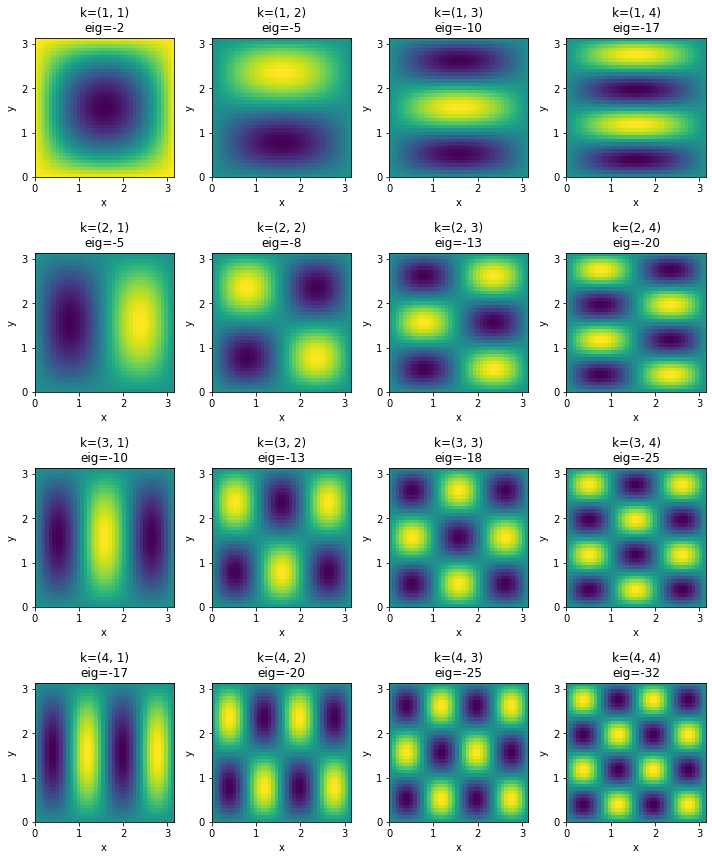
\includegraphics[width=0.9\textwidth]{figures/eigenfluids/16_basis_fields.png}
    \caption{Visualizing the curl of the first $16$ $\Phi_{\vb{k}}$ basis fields
    (i.e. $\phi_{\vb{k}}$), sampled on a $40 \times 40$ grid in our simulation
  domain $D = [0,\pi] \times [0,\pi]$.  Larger magnitudes of eigenvalues
correspond to smaller scale vortices.}
\end{figure}


%\label{page:last}
\end{document}
